\part{Ubetinget Optimering}
\label{part:unconstrained_optimization}

Ubetinget optimalisering (eller fri optimalisering) refererer til problemer uten eksplisitte restriksjoner på variablene \(\symbf{x}\), eller løsningsmengden \(\Omega\).
Dette betyr at vi kan søke etter løsninger i hele \(\Omega = \R^n\) uten å måtte ta hensyn til begrensninger som kan hindre oss i å finne den beste løsningen.

\chapter{Inntroduksjon til Ubetinget Optimalisering}
\label{chap:unconstrained_optimization}

\section{Definisjon og Problemstilling}
Vi fokuserer nå på problemet med å minimere en \textit{objektfunksjon}
\( f : \R^n \to \R \) over hele rommet \(\R^n\):

\[
	\min_{\symbf{x} \in \R^n} f(\symbf{x}) \tag{P} \label{eq:global_minimization_problem}
\]

Den tillatte løsningsmengden omfatter hele \( \Omega = \R^n\).
Siden det ikke finnes restriksjoner å ta hensyn til, blir både problemet og løsningsmetodene enklere sammenlignet med betingede optimeringsproblemer.

Vi fokuserer hovedsakelig på minimering, men alle metoder kan anvendes på maksimeringsproblemer ved å minimere \(-f(\symbf{x})\), siden \(\max_{\symbf{x}} f(\symbf{x}) = -\min_{\symbf{x}} (-f(\symbf{x}))\).

\subsection{Motivasjon og Anvendelser}
Ubetinget optimering oppstår naturlig i mange praktiske problemer:

\begin{itemize}
	\item \textbf{Tilpasning av modeller til data} (kurvetilpasning, regresjonsanalyse)
	\item \textbf{Maskinlæring} (trening av nevrale nettverk, logistisk regresjon)
	\item \textbf{Vitenskapelige beregninger} (simulering, minste kvadraters metode)
	\item \textbf{Bildebehandling} (filtrering, rekonstruksjon)
	\item \textbf{Økonomisk optimering} (porteføljeoptimering, kostnadsminimering)
\end{itemize}

I mange tilfeller kan også betingede optimeringsproblemer omformuleres som ubetingede problemer ved hjelp av straffefunksjoner eller barrierefunksjoner.

\section{Grunnleggende Konsepter}

\subsection{Lokale og Globale Optima}

Et viktig skille i optimeringsteori er mellom lokale og globale optima.

\begin{definition}{Globalt minimum}{global_minimum}
	Et punkt \(\symbf{x}^\ast \in \R^n\) er et \textit{globalt minimum} for funksjonen \(f\) hvis
	\[
		f(\symbf{x}^\ast) \leq f(\symbf{x}) \quad \text{for alle} \quad \symbf{x} \in \R^n
	\]
\end{definition}

\begin{definition}{Lokalt minimum}{local_minimum}
	Et punkt \(\symbf{x}^\ast \in \R^n\) er et \textit{lokalt minimum} for funksjonen \(f\) hvis det finnes en åpen omegn \(U\) rundt \(\symbf{x}^\ast\) slik at
	\[
		f(\symbf{x}^\ast) \leq f(\symbf{x}) \quad \text{for alle} \quad \symbf{x} \in U
	\]
\end{definition}

Vi sier at minimumet er \textit{strengt} hvis ulikhetene over holder strengt for alle $\symbf{x} \neq \symbf{x}^\ast$.

\begin{figure}[h]
	\centering
	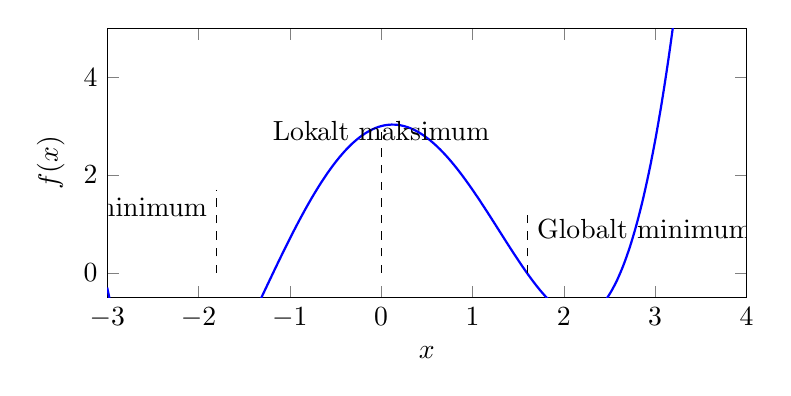
\begin{tikzpicture}
		\begin{axis}[
				xlabel={$x$},
				ylabel={$f(x)$},
				xmin=-3, xmax=4,
				ymin=-0.5, ymax=5,
				samples=100,
				smooth,
				domain=-3:4,
				width=0.8\textwidth,
				height=5cm
			]
			\addplot[blue, thick] {0.2*x^4-2*x^2+0.5*x+3};
			\draw[dashed] (axis cs:-1.8,0) -- (axis cs:-1.8,1.7);
			\draw[dashed] (axis cs:1.6,0) -- (axis cs:1.6,1.2);
			\draw[dashed] (axis cs:0,0) -- (axis cs:0,3);

			\node at (axis cs:-1.8,1.35) [anchor=east] {Lokalt minimum};
			\node at (axis cs:1.6,0.9) [anchor=west] {Globalt minimum};
			\node at (axis cs:0,3.3) [anchor=north] {Lokalt maksimum};
		\end{axis}
	\end{tikzpicture}
	\caption{Eksempel på en funksjon med både lokale og globale ekstremalpunkter}
	\label{fig:local_vs_global}
\end{figure}

Figur \ref{fig:local_vs_global} viser en funksjon med både lokale og globale ekstremalpunkter. I praksis er det generelt vanskelig å garantere at et funnet minimum er globalt, spesielt for ikke-konvekse funksjoner.

\subsection{Stasjonære Punkter}

For differensierbare funksjoner er et nødvendig vilkår for et lokalt minimum at gradienten er null.

\begin{definition}{Stasjonært punkt}{stationary_point}
	Et punkt \(\symbf{x}^\ast \in \R^n\) kalles et \textit{stasjonært punkt} for \(f\) hvis \(f\) er differensierbar ved \(\symbf{x}^\ast\) og
	\[
		\nabla f(\symbf{x}^\ast) = \symbf{0}
	\]
\end{definition}

Stasjonære punkter kan være:
\begin{itemize}
	\item Lokale minima
	\item Lokale maksima
	\item Sadelpunkter
\end{itemize}

For å skille mellom disse typene, bruker vi andreordens informasjon.

\subsection{Konveksitet}

Konvekse funksjoner spiller en spesiell rolle i optimering fordi lokale minima også er globale minima.

\begin{definition}{Konveks funksjon}{convex_function}
	En funksjon \(f: \R^n \to \R\) er \textit{konveks} hvis for alle \(\symbf{x}, \symbf{y} \in \R^n\) og alle \(\lambda \in [0,1]\) gjelder
	\[
		f(\lambda \symbf{x} + (1-\lambda)\symbf{y}) \leq \lambda f(\symbf{x}) + (1-\lambda)f(\symbf{y})
	\]
	Funksjonen er \textit{strengt konveks} hvis ulikheten over er streng for alle \(\symbf{x} \neq \symbf{y}\) og \(\lambda \in (0,1)\).
\end{definition}

For differensierbare funksjoner har vi følgende karakterisering:

\begin{proposition}{Karakterisering av differensierbare konvekse funksjoner}{differentiable_convex}
	La \(f: \R^n \to \R\) være en differensierbar funksjon. Da er \(f\) konveks hvis og bare hvis for alle \(\symbf{x}, \symbf{y} \in \R^n\) gjelder
	\[
		f(\symbf{y}) \geq f(\symbf{x}) + \nabla f(\symbf{x})^T (\symbf{y} - \symbf{x})
	\]
\end{proposition}

For to ganger differensierbare funksjoner har vi en enda enklere karakterisering:

\begin{proposition}{Karakterisering med Hesse-matrisen}{hessian_convex}
	La \(f: \R^n \to \R\) være to ganger kontinuerlig differensierbar. Da er \(f\) konveks hvis og bare hvis Hesse-matrisen \(\nabla^2 f(\symbf{x})\) er positiv semidefinit for alle \(\symbf{x} \in \R^n\).

	Funksjonen er strengt konveks hvis og bare hvis Hesse-matrisen er positiv definit for alle \(\symbf{x} \in \R^n\).
\end{proposition}

\section{Optimalitetskriterier}

\subsection{Førsteordens Nødvendige Betingelse}

\begin{theorem}{Førsteordens nødvendige betingelse}{first_order_necessary}
	Anta at \(f: \R^n \to \R\) er kontinuerlig differensierbar og at \(\symbf{x}^\ast\) er et lokalt minimum for \(f\). Da er \(\symbf{x}^\ast\) et stasjonært punkt, dvs.
	\[
		\nabla f(\symbf{x}^\ast) = \symbf{0}
	\]
\end{theorem}

\subsection{Andreordens Betingelser}

\begin{theorem}{Andreordens nødvendige betingelse}{second_order_necessary}
	Anta at \(f: \R^n \to \R\) er to ganger kontinuerlig differensierbar og at \(\symbf{x}^\ast\) er et lokalt minimum for \(f\). Da er Hesse-matrisen \(\nabla^2 f(\symbf{x}^\ast)\) positiv semidefinit.
\end{theorem}

\begin{theorem}{Andreordens tilstrekkelig betingelse}{second_order_sufficient}
	Anta at \(f: \R^n \to \R\) er to ganger kontinuerlig differensierbar, \(\nabla f(\symbf{x}^\ast) = \symbf{0}\) og Hesse-matrisen \(\nabla^2 f(\symbf{x}^\ast)\) er positiv definit. Da er \(\symbf{x}^\ast\) et strengt lokalt minimum for \(f\).
\end{theorem}

\section{Konvergens og Konvergenshastighet \texorpdfstring{\(\symbf{x}_k \to \symbf{x}^\ast\)}{x\_k to x\_ast}}
\label{sec:convergence}

I studiet av numeriske metoder for ubetinget optimering er det viktig å forstå både om og hvor raskt metodene konvergerer. Vi definerer ulike typer konvergensrater:

\begin{definition}{Konvergensrater}{convergence_rates}
	Anta at sekvensen \(\{\symbf{x}_k\}\) konvergerer mot \(\symbf{x}^\ast\). Vi sier at konvergensen er:
	\begin{itemize}
		\item \textbf{Lineær} hvis det finnes en konstant \(r \in (0,1)\) slik at
		      \[
			      \lim_{k \to \infty} \frac{\|\symbf{x}_{k+1} - \symbf{x}^\ast\|}{\|\symbf{x}_k - \symbf{x}^\ast\|} = r
		      \]

		\item \textbf{Superlineær} hvis
		      \[
			      \lim_{k \to \infty} \frac{\|\symbf{x}_{k+1} - \symbf{x}^\ast\|}{\|\symbf{x}_k - \symbf{x}^\ast\|} = 0
		      \]

		\item \textbf{Kvadratisk} hvis det finnes en konstant \(M > 0\) slik at
		      \[
			      \lim_{k \to \infty} \frac{\|\symbf{x}_{k+1} - \symbf{x}^\ast\|}{\|\symbf{x}_k - \symbf{x}^\ast\|^2} = M
		      \]
	\end{itemize}
\end{definition}

Kvadratisk konvergens betyr i praksis at antall korrekte sifre omtrent dobles i hver iterasjon, mens lineær konvergens betyr at antall korrekte sifre øker med en konstant for hver iterasjon.

\begin{figure}[h]
	\centering
	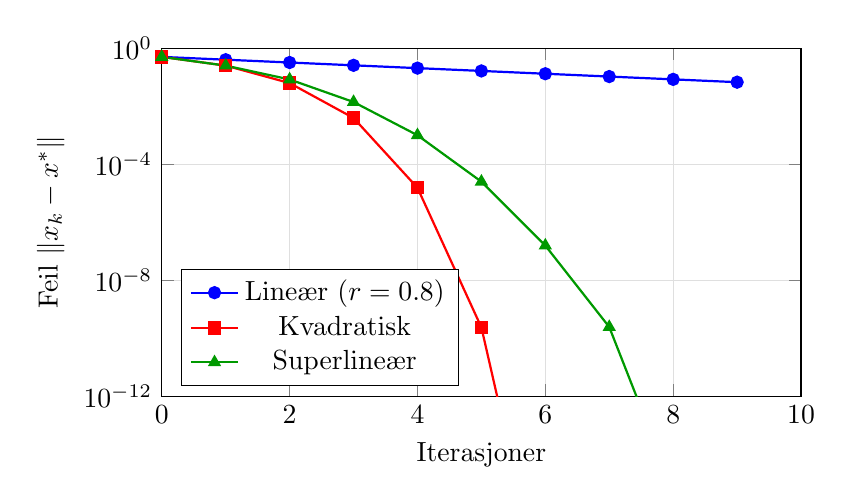
\begin{tikzpicture}
		\begin{semilogyaxis}[
				xlabel={Iterasjoner},
				ylabel={Feil $\|\symbf{x}_k - \symbf{x}^\ast\|$},
				xmin=0, xmax=10,
				ymin=1e-12, ymax=1,
				width=0.8\textwidth,
				height=6cm,
				legend pos=south west,
				grid=both,
				minor grid style={gray!25},
				major grid style={gray!25}
			]
			\addplot[blue, thick, mark=*] coordinates {
					(0, 0.5)
					(1, 0.4)
					(2, 0.32)
					(3, 0.256)
					(4, 0.2048)
					(5, 0.16384)
					(6, 0.131072)
					(7, 0.1048576)
					(8, 0.08388608)
					(9, 0.067108864)
				};
			\addlegendentry{Lineær ($r=0.8$)}

			\addplot[red, thick, mark=square*] coordinates {
					(0, 0.5)
					(1, 0.25)
					(2, 0.0625)
					(3, 0.00390625)
					(4, 1.52588e-5)
					(5, 2.32831e-10)
					(6, 5.42101e-20)
					(7, 2.93873e-39)
					(8, 8.63617e-78)
					(9, 7.45832e-155)
				};
			\addlegendentry{Kvadratisk}

			\addplot[green!60!black, thick, mark=triangle*] coordinates {
					(0, 0.5)
					(1, 0.25)
					(2, 0.0833333)
					(3, 0.0138889)
					(4, 0.000992063)
					(5, 2.48016e-5)
					(6, 1.55009e-7)
					(7, 2.40637e-10)
					(8, 5.79065e-16)
					(9, 3.35458e-27)
				};
			\addlegendentry{Superlineær}

		\end{semilogyaxis}
	\end{tikzpicture}
	\caption{Sammenligning av konvergensrater: lineær, superlineær og kvadratisk konvergens}
	\label{fig:convergence_rates}
\end{figure}

Figur \ref{fig:convergence_rates} illustrerer ulike konvergensrater. Bemerk at en logaritmisk skala brukes på y-aksen for å bedre visualisere de dramatiske forskjellene i konvergenshastighet.

I de påfølgende kapitler vil vi studere numeriske metoder for å løse ubetingede optimeringsproblemer og analysere deres konvergensegenskaper.

\chapter{Gradient metoder}
\label{chap:gradient_based_methods}
Gradientbaserte metoder er en klasse av numeriske algoritmer som benytter gradienten til objektfunksjonen for å finne minimum eller maksimum.
Disse metodene kan kategoriseres etter hvilken ordens derivert de bruker:

\begin{itemize}
	\item \textbf{Førsteordens metoder}: Bruker bare gradientinformasjon (f.eks. Steepest Descent)
	\item \textbf{Andreordens metoder}: Bruker både gradient og Hesse-matrise (f.eks. Newtons metode)
\end{itemize}

Man klassifiserer også gradientbaserte metoder i to hovedkategorier, \emph{linjesøkmetoder} og \emph{trust region-metoder}.
I linjesøkmetoder bestemmer vi først søkeretningen, deretter hvor langt vi skal gå i den retningen.
I trust region-metoder bestemmer vi først hvor langt vi kan gå (trust region-radiusen), deretter bestemmer vi både retning og steglengde samtidig.

\begin{forest}
	for tree={
	align=center,
	parent anchor=south,
	child anchor=north
	}
	[Gradientbaserte\\ metoder
		[Førsteordens\\ metoder
				[Steepest\\ Descent]
				[Konjugert\\ Gradient]
		]
		[Andreordens\\ metoder
				[Newtons\\ metode]
				[Quasi-Newton\\ metoder]
		]
	]
\end{forest}

\medskip
Både første- og andreordens metoder kan implementeres med enten linjesøk eller trust region strategier.
\section{Steepest Descent}\label{sec:steepest_descent}
Steepest Descent en en enkel metode for å minimere \(f: \mathbb{R}^n \to \mathbb{R}\) ved å følge den bratteste nedstigningsretningen \( \symbf{d}_k = -\nabla f(\symbf{x}_k)\) fra et gitt punkt \( \symbf{x}_k \).
\begin{definition}{Steepest Descent}{steepest_descent}
	Steepest Descent-algoritmen oppdaterer iterasjonen \( \symbf{x}_k \) ved å ta et skritt i retning av den negative gradienten:
	\[
		\symbf{x}_{k+1} = \symbf{x}_k + \alpha_k \symbf{d}_k,
	\]
	hvor \( \alpha_k > 0 \) er skrittlengden og \( \symbf{d}_k = -\nabla f(\symbf{x}_k) \) er nedstigningsretningen.
	\medskip
	Steepest Descent-algoritmen kan skrives som:
	\begin{align*}
		\symbf{x}_{k+1} & = \symbf{x}_k + \alpha_k \symbf{d}_k, \\
		\symbf{d}_k     & = -\nabla f(\symbf{x}_k).
	\end{align*}

\end{definition}

\begin{equation}
	\symbf{d}_k = -\nabla f(\symbf{x}_k),
\end{equation}
hvor \(\symbf{d}_k\) er nedstigningsretningen ved iterasjon \(k\).
\subsection{Steepest Descent Algoritme}
\begin{algorithm}[H]
	\SetAlgoLined
	\KwIn{Startpunkt \( \symbf{x}_0 \), toleranse \( \epsilon \), maks antall iterasjoner \( K \)}
	\KwOut{Omtrentelig løsning \( \symbf{x}^\ast \)}
	\For{\( k = 0, 1, 2, \ldots, K\)}{
		\(\symbf{d}_k = -\nabla f(\symbf{x}_k)\)\;
		Finn skrittlengde \(\alpha_k\) (f.eks.\ ved linjesøk-metode)\;
		\(\symbf{x}_{k+1} = \symbf{x}_k + \alpha_k \symbf{d}_k\)\;
		\If{\(\|\nabla f(\symbf{x}_{k+1})\| < \epsilon\)}{
			\Return \(\symbf{x}_{k+1}\)\;
		}
	}
	\caption{Steepest Descent}
	\label{alg:steepest_descent}
\end{algorithm}

\subsection{Konvergens av Steepest Descent}
Anta ett ideelt tilfelle der \(f\) er en kvadratisk funksjon, med en positiv definit og symmetrisk Hesse-matrise \(Q\), hvor objektfunksjonen er kvadratisk og linjesøkene er eksakte.
\begin{align*}
	f(\symbf{x})        & = \frac{1}{2} \symbf{x}^T Q \symbf{x} - \symbf{b}^T \symbf{x} \\
	\nabla f(\symbf{x}) & = Q \symbf{x} - \symbf{b}
\end{align*}\label{eq:quadratic_function}

hvor det minste punkt \(\symbf{x}^\ast\) er en unik løsning av
\[
	Q \symbf{x}^\ast = \symbf{b}.
\]
Da kan vi finne den beste steglengden \(\alpha_k\) som minimerer \(f(\symbf{x}_k - \alpha \nabla f(\symbf{x}_k))\) ved å derivere den med hensyn til \(\alpha\) og sette den lik null:
\begin{align*}
	f(\symbf{x}_k - \alpha \nabla f(\symbf{x}_k)) & = \frac{1}{2} (\symbf{x}_k - \alpha \nabla f(\symbf{x}_k))^T Q (\symbf{x}_k - \alpha \nabla f(\symbf{x}_k)) - \symbf{b}^T (\symbf{x}_k - \alpha \nabla f(\symbf{x}_k)), \\
	\frac{\partial f}{\partial \alpha}            & = -\nabla f(\symbf{x}_k)^T Q \symbf{x}_k + \alpha \nabla f(\symbf{x}_k)^T Q \nabla f(\symbf{x}_k) + \nabla f(\symbf{x}_k)^T \nabla f(\symbf{x}_k).
\end{align*}
Med å løse \(\frac{\partial f}{\partial \alpha} = 0\) for \(\alpha_k\) får vi:

\[
	\alpha_k = \frac{\nabla f_k^\top \nabla f_k}{\nabla f_k^\top Q \nabla f_k}
\]

Det gir oss den eksakte optimale steglengden \(\alpha_k\) for Steepest Descent-algoritmen.
\begin{equation*}
	\symbf{x}_{k+1} = \symbf{x}_k - \alpha_k \nabla f(\symbf{x}_k) = \symbf{x}_k - \left(\frac{\nabla f_k^\top \nabla f_k}{\nabla f_k^\top Q \nabla f_k}\right) \nabla f_k
\end{equation*}\label{eq:steepest_descent_update}
\subsection{Konvergenshastighet for Steepest Descent}
For å analysere konvergenshastigheten til Steepest Descent-algoritmen, vil vi undersøke hvordan feilen reduseres for hver iterasjon. Vi fokuserer først på det kvadratiske tilfellet med en positiv definit Hesse-matrise $Q$.

La oss definere feilen ved iterasjon $k$ som $\symbf{e}_k = \symbf{x}_k - \symbf{x}^\ast$, der $\symbf{x}^\ast$ er den eksakte løsningen. For en kvadratisk funksjon gjelder følgende forhold:
\[
	\frac{1}{2} \|\symbf{e}_k\|_Q^2 = \frac{1}{2} \|\symbf{x}_k - \symbf{x}^\ast\|_Q^2 = f(\symbf{x}_k) - f(\symbf{x}^\ast).
\]

Med eksakt linjesøk kan vi, basert på oppdateringsformelen~\eqref{eq:steepest_descent_update}, vise at feilen avtar lineært:
\[
	\|\symbf{e}_{k+1}\|_Q^2 = (1 - C) \|\symbf{e}_k\|_Q^2,
\]
hvor reduksjonsfaktoren $C$ er gitt ved:
\[
	C = \frac{[\nabla f_k^\top \nabla f_k]^2}{(\nabla f_k^\top Q \nabla f_k)(\nabla f_k^\top Q^{-1} \nabla f_k)}.
\]

Dette uttrykket kan være komplisert å beregne direkte, men vi kan etablere en øvre grense ved hjelp av kondisjonstallet til $Q$:

\begin{theorem}{Konvergenshastighet for Steepest Descent}{steepest_descent_convergence}
	Når Steepest Descent-metoden med eksakte linjesøk anvendes på en sterkt konveks kvadratisk funksjon~\eqref{eq:quadratic_function}, er konvergenshastigheten begrenset av:
	\[
		\norm{\symbf{x}_{k+1} - \symbf{x}^\ast}_Q^2 \leq \left(\frac{\kappa - 1}{\kappa + 1}\right)^2 \norm{\symbf{x}_k - \symbf{x}^\ast}_Q^2,
	\]
	hvor $\kappa = \frac{\lambda_n}{\lambda_1}$ er kondisjonstallet til $Q$, med $0 < \lambda_1 \leq \lambda_2 \leq \cdots \leq \lambda_n$ som egenverdiene til $Q$.
\end{theorem}

Dette resultatet viser at konvergenshastigheten til Steepest Descent i stor grad avhenger av kondisjonstallet $\kappa$. Når $\kappa$ er stort (dårlig kondisjonert problem), nærmer faktoren $\frac{\kappa - 1}{\kappa + 1}$ seg 1, hvilket resulterer i svært langsom konvergens.

For den generelle, ikke-kvadratiske situasjonen kan vi forvente lignende lineær konvergensatferd nær løsningen, men med konstanten bestemt av kondisjonstallet til Hesse-matrisen ved løsningspunktet.

En detaljert utledning av dette resultatet finnes i \cite{luenberger1984linear}.

\subsection{Konvergens ved generelle funksjoner}
For generelle, ikke-kvadratiske funksjoner \(f : \mathbb{R}^n \to \mathbb{R}\), gjelder fremdeles en lineær konvergensrate for Steepest Descent-metoden dersom \(f\) er to ganger kontinuerlig deriverbar og linjesøket er eksakt.
Men man kan fortsatt vise at konvergenshastigheten i nærheten av en løsning \(x^\ast\) fortsatt begrenses av kondisjonstallet til Hesse-matrisen.

\begin{theorem}{Asymptotisk konvergens av Steepest Descent}{steepest_descent_general}
	Anta at \(f : \mathbb{R}^n \to \mathbb{R}\) er to ganger kontinuerlig deriverbar og at iteratene \(\symbf{x}_k\) generert av Steepest Descent med eksakt linjesøk konvergerer til et punkt \(x^\ast\), hvor Hesse-matrisen \(\nabla^2 f(x^\ast)\) er positiv definit.

	La \(\lambda_1 \leq \lambda_2 \leq \cdots \leq \lambda_n\) være egenverdiene til \(\nabla^2 f(x^\ast)\). Da finnes det en konstant \(r \in \left( \frac{\lambda_n - \lambda_1}{\lambda_n + \lambda_1}, 1 \right)\) slik at
	\[
		f(x_{k+1}) - f(x^\ast) \leq r^2 \left[ f(x_k) - f(x^\ast) \right]
	\]
	for alle tilstrekkelig store \(k\).
\end{theorem}

Dette viser at metoden har \emph{lineær konvergens}, men at konvergensfaktoren \(r^2\) nærmer seg 1 når kondisjonstallet \(\kappa = \lambda_n / \lambda_1\) blir stort. Dette innebærer at selv under ideelle forhold (eksakt linjesøk og glatt funksjon), kan Steepest Descent konvergere ekstremt langsomt. For eksempel, hvis \(\kappa = 800\) og startverdien er \(f(x_1) = 1\), kan man etter 1000 iterasjoner fortsatt ha

\section{Newtons Metode}
\label{sec:newtons_method}
Newtons metode er en iterativ metode for å finne stasjonære punkter (typisk minima eller maxima) av glatt funksjoner.
\[
	\mathbf{x}_{k+1} = \mathbf{x}_k - [\nabla^2 f(\mathbf{x}_k)]^{-1} \nabla f(\mathbf{x}_k) = \mathbf{x}_k - \alpha_k \mathbf{d}_k
\]\label{eq:newtons_method}

Den bruker 2. Ordens Taylor-approksimasjoner av objektfunksjonen, og bruker både gradienten og Hesse-matrisen $H$ til å finne en retning $\symbf{d}_k$ for å oppdatere iterasjonen $\symbf{x}_k$.

\[
	\symbf{d}_k = -[\nabla^2 f(\symbf{x}_k)]^{-1} \nabla f(\symbf{x}_k) = -\symbf{H}^{-1} \nabla f(\symbf{x}_k)
\]

Ulempen er at metoden krever at man finner Hesse-matrisen $H$, og regner ut dens inverse $H^{-1}$, noe som kan være kostbart i høyere dimensjoner.

Under visse regularitetsforutsetninger kan metoden konvergere med kvadratisk hastighet $\norm{e}_{k+1} \leq C \norm{e_k}^2$, noe som gjør den vesentlig mer effektiv enn førsteordens metoder i nærhet av løsningen.
Med regularitetsforutsetninger menes at objektfunksjonen $f$ er to ganger kontinuerlig deriverbar, og at Hesse-matrisen $\nabla^2 f(x^\ast)$ ved løsningen $x^\ast$ er positiv definit.
Disse forutsetningene sikrer at metoden kan utnytte kurvaturinformasjonen i $f$ for raskere konvergens.

\[
	\norm{\symbf{e}_{k+1}} \leq C \norm{\symbf{e}_k}^2 \approx \mathcal{O}(\norm{\symbf{e}_k}^2)
\]

\subsection{Newtons Metode Algoritme}
Skrittlengden \(\alpha_k\) kan bestemmes ved linjesøk, eller andre metoder for å minimere \(f(\symbf{x}_k + \alpha \symbf{d}_k)\) i retning av \(\symbf{d}_k\).

\begin{algorithm}[H]
	\SetAlgoLined
	\KwIn{Startpunkt \( \symbf{x}_0 \), tol. \( \epsilon > 0 \), maks iter. \( K_{max} \)}
	\KwOut{Løsning \( \approx \symbf{x}^\ast \)}
	Start Skritt \(\alpha_0 = 1\)\;
	\For{\( k = 0, 1, 2, \ldots, K_{max}\)}{
	\(\symbf{d}_k = -[\nabla^2 f(\symbf{x}_k)]^{-1}\,\nabla f(\symbf{x}_k)\)\;
	Finn Ny Skritt \(\alpha_k\) (f.eks.\ ved linjesøk-metoder)\;
	\(\symbf{x}_{k+1} = \symbf{x}_k + \alpha_k \symbf{d}_k\)\;
	\If{\(\|\nabla f(\symbf{x}_{k+1})\| < \epsilon\)}{
		\Return \(\symbf{x}_{k+1}\)\;
	}
	}
	\caption{Newtons metode}
\end{algorithm}

\subsection{Konvergens av Newtons Metode}
Newtons metode kan konvergere lokalt kvadratisk under visse forutsetninger.
La \( f : \mathbb{R}^n \to \mathbb{R} \) være to ganger kontinuerlig deriverbar. Anta at:

\begin{enumerate}
	\item Det finnes et \(\symbf{x}^\ast\) slik at \(\nabla f(\symbf{x}^\ast) = 0\).
	\item Hesse-matrisen \(\nabla^2 f(\symbf{x}^\ast)\) er regulær (invertibel).
	\item \(\nabla^2 f\) er Lipschitz-kontinuerlig i et nabolag rundt \(\symbf{x}^\ast\); dvs.\ det finnes \( L > 0 \) slik at
	      \[
		      \| \nabla^2 f(\symbf{x}) - \nabla^2 f(\symbf{y}) \|
		      \;\le\;
		      L\,\|\symbf{x} - \symbf{y}\|,
	      \]
	      for alle \(\symbf{x}, \symbf{y}\) i dette nabolaget.
\end{enumerate}

Da kan man vise at for en startverdi \(\symbf{x}_0\) nær \(\symbf{x}^\ast\), vil Newtons metode konvergere kvadratisk mot \(\symbf{x}^\ast\).
Beviset forutsetter at startverdien \(\symbf{x}_0\) er tilstrekkelig nær \(\symbf{x}^\ast\). I praksis benyttes ofte modifikasjoner, som for eksempel \textit{dempet Newton} (med linjesøk), for å sikre global konvergens før man oppnår den raske, lokale konvergensfasen.
\begin{proof}{}{}
	La \(\symbf{e}_k = \symbf{x}_k - \symbf{x}^\ast\) være feilen ved iterasjon \(k\).
	Ved Taylor-utvidelse av gradienten får vi:
	\[
		\nabla f(\symbf{x}_k)
		= \nabla^2 f(\symbf{x}^\ast)\,(\symbf{x}_k - \symbf{x}^\ast) + r(\symbf{x}_k),
	\]
	hvor \(\|r(\symbf{x}_k)\|\) er \(\mathcal{O}(\|\symbf{e}_k\|^2)\). Newtons oppdateringsregel er
	\[
		\symbf{x}_{k+1}
		= \symbf{x}_k
		- [\nabla^2 f(\symbf{x}_k)]^{-1}\,\nabla f(\symbf{x}_k).
	\]
	I et lite nabolag av \(\symbf{x}^\ast\) kan vi anta at
	\(\nabla^2 f(\symbf{x}_k)\approx \nabla^2 f(\symbf{x}^\ast)\), slik at
	\[
		\symbf{e}_{k+1}
		\;=\; \symbf{x}_{k+1} - \symbf{x}^\ast
		\;\approx\;
		-[\nabla^2 f(\symbf{x}^\ast)]^{-1}\,r(\symbf{x}_k).
	\]
	Dermed blir
	\[
		\|\symbf{e}_{k+1}\| \lesssim \|[\nabla^2 f(\symbf{x}^\ast)]^{-1}\| \|r(\symbf{x}_k)\| \le C \|\symbf{e}_k\|^2
	\]
	for en konstant \(C>0\). Dette illustrerer \textit{kvadratisk konvergens} når \(\symbf{x}_0\) er nært \(\symbf{x}^\ast\).
\end{proof}

\subsection{Egenskaper}
\begin{itemize}
	\item \textbf{Kvadratisk konvergens}: Under gitte forutsetninger dobles antall riktige sifre omtrent for hver iterasjon.
	\item \textbf{Krever andreordens deriverbarhet}: \(\nabla^2 f(\symbf{x})\) må eksistere og være invertibel.
	\item \textbf{Beregning kan være kostbar}: Å beregne og invertere \(\nabla^2 f(\symbf{x})\) er dyrt, spesielt i store dimensjoner.
	\item \textbf{Global vs.\ lokal konvergens}: Metoden garanterer ikke nødvendigvis global konvergens uten videre tiltak.
\end{itemize}

\subsection{Varianter av Newtons metode}
\begin{itemize}
	\item \textbf{Dempet Newtons metode}: Benytter en skrittlengde \(\alpha_k\) (linjesøk) for å unngå for store steg.
	\item \textbf{Kvasi-Newton-metoder}: Reduserer kostnader ved å approksimere Hesse-matrisen (f.eks.\ BFGS, DFP).
\end{itemize}

\section{Konjugert Gradientmetoden}
\label{sec:conjugate_gradient}

Konjugert Gradient (CG) metoden er en effektiv iterativ algoritme for å løse lineære ligningssystemer og optimere kvadratiske funksjoner. Den er spesielt nyttig for store, men sparse systemer.

\subsection{Grunnleggende Konsept}
CG-metoden genererer en sekvens av retninger som er konjugerte med hensyn til en symmetrisk, positiv definit matrise. For en kvadratisk funksjon:
\[
	f(\symbf{x}) = \frac{1}{2}\symbf{x}^T\symbf{A}\symbf{x} - \symbf{b}^T\symbf{x} + c,
\]
hvor \(\symbf{A}\) er symmetrisk, positiv definit, søker CG-metoden å løse \(\nabla f(\symbf{x}) = \symbf{A}\symbf{x} - \symbf{b} = \symbf{0}\).

\subsection{CG-algoritme}

\begin{algorithm}[H]
	\SetAlgoLined
	\KwIn{Startpunkt \(\symbf{x}_0\), toleranse \(\epsilon > 0\)}
	\KwOut{Omtrentelig løsning \(\symbf{x}^\ast\)}
	\(\symbf{r}_0 \gets \symbf{b} - \symbf{A}\symbf{x}_0\) \tcc*{Residual}
	\(\symbf{p}_0 \gets \symbf{r}_0\) \tcc*{Første søkeretning}
	\For{\(k = 0, 1, 2, \ldots\)}{
		\If{\(\|\symbf{r}_k\| < \epsilon\)}{
			\Return \(\symbf{x}_k\) \tcc*{Konvergens oppnådd}
		}
		\(\alpha_k \gets \frac{\symbf{r}_k^T\symbf{r}_k}{\symbf{p}_k^T\symbf{A}\symbf{p}_k}\) \tcc*{Optimal skrittlengde}
		\(\symbf{x}_{k+1} \gets \symbf{x}_k + \alpha_k\symbf{p}_k\) \tcc*{Oppdater løsning}
		\(\symbf{r}_{k+1} \gets \symbf{r}_k - \alpha_k\symbf{A}\symbf{p}_k\) \tcc*{Oppdater residual}
		\(\beta_{k+1} \gets \frac{\symbf{r}_{k+1}^T\symbf{r}_{k+1}}{\symbf{r}_k^T\symbf{r}_k}\) \tcc*{Konjugasjonsparameter}
		\(\symbf{p}_{k+1} \gets \symbf{r}_{k+1} + \beta_{k+1}\symbf{p}_k\) \tcc*{Ny søkeretning}
	}
	\caption{Konjugert Gradient Metode (CG)}
\end{algorithm}

\subsection{Ikke-lineær Konjugert Gradient Metode (Non-Linear CG)}

For generelle ikke-lineære funksjoner tilpasses algoritmen:

\begin{algorithm}[H]
	\SetAlgoLined
	\KwIn{Startpunkt \(\symbf{x}_0\), toleranse \(\epsilon > 0\)}
	\KwOut{Omtrentelig løsning \(\symbf{x}^\ast\)}
	\(\symbf{g}_0 \gets \nabla f(\symbf{x}_0)\) \tcc*{Gradient}
	\(\symbf{p}_0 \gets -\symbf{g}_0\) \tcc*{Første søkeretning}
	\For{\(k = 0, 1, 2, \ldots\)}{
		\If{\(\|\symbf{g}_k\| < \epsilon\)}{
			\Return \(\symbf{x}_k\) \tcc*{Konvergens oppnådd}
		}
		Finn \(\alpha_k\) ved linjesøk som minimerer \(f(\symbf{x}_k + \alpha\symbf{p}_k)\) \;
		\(\symbf{x}_{k+1} \gets \symbf{x}_k + \alpha_k\symbf{p}_k\) \tcc*{Oppdater løsning}
		\(\symbf{g}_{k+1} \gets \nabla f(\symbf{x}_{k+1})\) \tcc*{Ny gradient}
		Beregn \(\beta_{k+1}\) \tcc*{f.eks. FR eller PR}\;
		\(\symbf{p}_{k+1} \gets -\symbf{g}_{k+1} + \beta_{k+1}\symbf{p}_k\) \tcc*{Ny søkeretning}
	}
	\caption{Ikke-lineær Konjugert Gradient Metode (Non-Linear CG)}
\end{algorithm}

\(\beta_{k+1}\) er konjugasjonsparameteren som bestemmer hvordan den nye søkeretningen \(\symbf{p}_{k+1}\) kombinerer den nåværende gradienten \(\symbf{g}_{k+1}\) med den forrige søkeretningen \(\symbf{p}_k\).
Intuitivt er egentlig \(\beta_{k+1}\) bare en vekt som bestemmer hvor mye av den forrige retningen \(\symbf{p}_k\) som skal beholdes i den nye retningen \(\symbf{p}_{k+1}\).

\subsection{Valg av \texorpdfstring{\(\beta\)}{beta}-parameter}
Det finnes flere metoder for å velge \(\beta_{k+1}\) i den ikke-lineære konjugerte gradientmetoden.

\subsubsection{Fletcher-Reeves (FR)}
Fletcher-Reeves oppdaterer \(\beta_{k+1}\) basert på forholdet mellom normene til gradientene i to påfølgende iterasjoner.
Dette sikrer at søkeretningene forblir konjugerte med hensyn til Hessian-matrisen for kvadratiske funksjoner.

\begin{definition}{Fletcher--Reeves}{fletcher_reeves}
	\[
		\beta_{k+1}^{FR} = \frac{\symbf{g}_{k+1}^T\symbf{g}_{k+1}}{\symbf{g}_k^T\symbf{g}_k} \tag{FR}
	\]
\end{definition}

\subsubsection{Polak--Ribière (PR)}
Polak--Ribière oppdaterer \(\beta_{k+1}\) basert på både normene til gradientene og forskjellen mellom gradientene i to påfølgende iterasjoner. Dette gir en mer dynamisk oppdatering sammenlignet med Fletcher--Reeves.
\begin{definition}{Polak-Ribière}{polak_ribiere}
	\[
		\beta_{k+1}^{PR} = \frac{\symbf{g}_{k+1}^T(\symbf{g}_{k+1}-\symbf{g}_k)}{\symbf{g}_k^T\symbf{g}_k} \tag{PR}
	\]
\end{definition}


\begin{remark}{Håndtering av negativ \(\beta_{k+1}^{PR}\)}{}
	Denne metoden kan gi raskere konvergens i praksis, men kan også føre til ustabilitet hvis \(\beta_{k+1}^{PR}\) blir negativ.
	I slike tilfeller kan \(\beta_{k+1}^{PR}\) settes til null for å sikre at algoritmen fortsatt fungerer som en gradientmetode.
\end{remark}

\subsubsection{Hestenes--Stiefel (HS)}
Hestenes--Stiefel oppdaterer \(\beta_{k+1}\) ved å bruke forholdet mellom gradientforskjellen og søkeretningen.
\begin{definition}{Hestenes--Stiefel}{hestenes_stiefel}
	\[
		\beta_{k+1}^{HS} = \frac{\symbf{g}_{k+1}^T(\symbf{g}_{k+1} - \symbf{g}_k)}{\symbf{p}_k^T(\symbf{g}_{k+1} - \symbf{g}_k)} \tag{HS}
	\]
\end{definition}
Hestenes--Stiefel-metoden kan være mer effektiv enn både Fletcher--Reeves og Polak--Ribière i visse tilfeller, spesielt når gradientforskjellene \(\symbf{g}_{k+1} - \symbf{g}_k\) er små, og søkeretningene \(\symbf{p}_k\) er godt tilpasset problemets kurvatur.
Dette skyldes at Hestenes--Stiefel-formelen tar hensyn til både gradientendringer og søkeretningens geometri, noe som kan gi en mer stabil oppdatering av \(\beta_{k+1}\).

\begin{remark}{Ustabilitet i Hestenes--Stiefel-metoden}{}
	En potensiell ulempe med Hestenes--Stiefel-metoden er at den kan bli ustabil hvis nevneren \(\symbf{p}_k^T(\symbf{g}_{k+1} - \symbf{g}_k)\) blir svært liten. For å unngå dette kan man bruke en modifisert versjon der \(\beta_{k+1}\) settes til null når ustabilitet oppdages.
\end{remark}

\begin{example}{}{}
	Anta at vi ønsker å minimere en kvadratisk funksjon \(f(\symbf{x}) = \frac{1}{2}\symbf{x}^\top A\symbf{x} - \symbf{b}^\top \symbf{x}\), der \(A\) er symmetrisk og positiv definit.
	\ref{def:hestenes_stiefel} kan gi raskere konvergens enn Fletcher--Reeves og Polak--Ribière hvis \(A\) har et høyt kondisjonstall \(\kappa(A)\), fordi den bedre utnytter informasjonen om gradientendringene.
\end{example}

Likevel kan den føre til ustabilitet hvis nevneren blir svært liten.
For å unngå dette kan man sette \(\beta_{k+1}^{HS} = 0\) når det er nødvendig for å opprettholde stabiliteten.

\subsection{Egenskaper}
\begin{itemize}
	\item \textbf{Rask konvergens for kvadratiske funksjoner:}
	      For kvadratiske funksjoner konvergerer metoden på maksimalt \(n\) iterasjoner.
	\item \textbf{Minneeffektivitet:}
	      Metoden lagrer kun et begrenset antall vektorer, noe som gjør den godt egnet for store problemer.
	\item \textbf{Numerisk stabilitet:}
	      Den er robust mot avrundingsfeil og opprettholder numerisk stabilitet, spesielt når periodiske omstarter benyttes.\footnote{Periodiske omstarter innebærer å tilbakestille algoritmen med jevne mellomrom for å reinitialisere retningene og sikre at de forblir ortogonale. Denne teknikken bidrar til å redusere akkumulerte beregningsfeil og opprettholder algoritmens effektivitet.}
	\item \textbf{Prekondisjonering:}
	      Metodens ytelse kan forbedres ytterligere ved å bruke en prekondisjonerer \(M\), som transformerer problemet for å akselerere konvergensen.
\end{itemize}

\subsection{Prekondisjonering}
Konvergenshastigheten kan forbedres ved å bruke en prekondisjonerer \(\symbf{M}\) som approksimerer \(\symbf{A}\) på en inverterbar måte. Den prekondisjonerte algoritmen løser det transformerte systemet:
\[
	\symbf{M}^{-1}\symbf{A}\symbf{x} = \symbf{M}^{-1}\symbf{b}.
\]
Dette reduserer kondisjonstallet \(\kappa(\symbf{M}^{-1}\symbf{A})\) og akselererer konvergensen.

\section{Quasi-Newton Metoder}
\label{sec:quasi_newton}

Quasi-Newton-metoder er en klasse av optimeringsalgoritmer utviklet for å løse ikke-lineære optimeringsproblemer. De bygger på ideene bak Newtons metode, men er spesielt nyttige når Hesse-matrisen \( \nabla^2 f(\symbf{x}) \) er vanskelig å beregne eller invertere.

Ettersom eksplisitt inversjon av Hesse-matrisen krever \( \mathcal{O}(n^2) \) lagring og \( \mathcal{O}(n^3) \) regneoperasjoner, blir Newtons metode ofte upraktisk i høyere dimensjoner.
Quasi-Newton-metoder unngår dette ved å iterativt lage en approksimasjon av Hesse-matrisen, eller dens invers, basert på gradientinformasjon fra tidligere iterasjoner.

Søkeretningen defineres da som
\[
	\symbf{p}_k = -B_k^{-1} \nabla f(\symbf{x}_k),
\]
der \( B_k \) er en symmetrisk og positivt definit matrise som approksimerer \( \nabla^2 f(\symbf{x}_k) \). Steglengden \( \alpha_k \) velges vanligvis gjennom linjesøk som tilfredsstiller Wolfe- eller sterke Wolfe-betingelser.

\subsection{Motivasjon}
Newtons metode krever eksplisitt beregning og inversjon av Hesse-matrisen \( \nabla^2 f(\symbf{x}) \) i hver iterasjon, noe som er kostbart i høyere dimensjoner.

Quasi-Newton-metoder reduserer denne kostnaden ved å:
\begin{itemize}
	\item Lage en iterativ approksimasjon av Hesse-matrisen (eller dens invers),
	\item Oppdatere denne approksimasjonen ved hjelp av gradientforskjeller fra tidligere iterasjoner,
	\item Unngå eksplisitt inversjon gjennom spesifikke oppdateringsformler.
\end{itemize}

\subsection{Algoritme for Quasi-Newton metoder}

\begin{algorithm}[H]
	\DontPrintSemicolon
	\KwIn{Startpunkt \( \mathbf{x}_0 \in \mathbb{R}^n \), toleranse \( \varepsilon > 0 \), initial matrise \( \mathbf{B}_0 \succ 0 \)}
	\KwOut{Omtrentlig løsning \( \mathbf{x}^\ast \)}

	\textbf{Initialiser:} \( k \gets 0 \)\;
	\While{\( \| \nabla f(\mathbf{x}_k) \| > \varepsilon \)}{
	Beregn søkeretning: \( \mathbf{p}_k = -\mathbf{B}_k^{-1} \nabla f(\mathbf{x}_k) \)\;

	Velg steglengde \( \alpha_k > 0 \) ved linjesøk (f.eks. Wolfe-betingelser)\;

	Oppdater iterasjon: \( \mathbf{x}_{k+1} = \mathbf{x}_k + \alpha_k \mathbf{p}_k \)\;

	Definer: \( \mathbf{s}_k = \mathbf{x}_{k+1} - \mathbf{x}_k \), \quad
	\( \mathbf{y}_k = \nabla f(\mathbf{x}_{k+1}) - \nabla f(\mathbf{x}_k) \)\;

	Oppdater \( \mathbf{B}_k \to \mathbf{B}_{k+1} \) ved bruk av f.eks. BFGS-oppdatering:\;
	\Indp
	\( \mathbf{B}_{k+1} = \mathbf{B}_k
	- \frac{\mathbf{B}_k \mathbf{s}_k \mathbf{s}_k^\top \mathbf{B}_k}{\mathbf{s}_k^\top \mathbf{B}_k \mathbf{s}_k}
	+ \frac{\mathbf{y}_k \mathbf{y}_k^\top}{\mathbf{y}_k^\top \mathbf{s}_k} \)\;
	\Indm

	\( k \gets k + 1 \)\;
	}

	\Return \( \mathbf{x}_k \)\;
	\caption{Quasi-Newton Metode}
	\label{alg:quasi_newton}
\end{algorithm}

\subsection{Sekantligningen}
For å oppdatere Hesse-approksimasjonen, må vi løse sekantligningen:
\[
	\symbf{B}_{k+1}\symbf{s}_k = \symbf{y}_k,
\]
Dette er en viktig del av Quasi-Newton-metodene, da den gir oss en måte å oppdatere Hesse-approksimasjonen på uten å måtte beregne den eksakte Hesse-matrisen.

I praksis jobber vi ofte direkte med den inverse approksimasjonen av Hesse-matrisen, \(\symbf{H}_k\), i stedet for \(\symbf{B}_k\). Dette er fordi det er mer numerisk stabilt og krever mindre minne.
\[
	\symbf{H}_k \approx [\nabla^2 f(\symbf{x}_k)]^{-1} =[\symbf{B}_k^{METODE}]^{-1}
\]

\subsection{Broyden-Fletcher-Goldfarb-Shanno (BFGS) oppdatering}
BFGS er en av de mest brukte Quasi-Newton-metodene.
Den oppdaterer den inverse Hesse-approksimasjonen ved å bruke gradientinformasjon fra to påfølgende iterasjoner.

\begin{definition}{BFGS-oppdatering}{bfgs_update}

	\begin{align*}
		\symbf{B}_{k+1}^{BFGS} & = \symbf{B}_k - \frac{\symbf{B}_k\symbf{s}_k\symbf{s}_k^T\symbf{B}_k}{\symbf{s}_k^T\symbf{B}_k\symbf{s}_k} + \frac{\symbf{y}_k\symbf{y}_k^T}{\symbf{y}_k^T\symbf{s}_k}                                                                          \\
		\symbf{H}_{k+1}        & = \left(\symbf{I} - \frac{\symbf{s}_k\symbf{y}_k^T}{\symbf{y}_k^T\symbf{s}_k}\right) \symbf{H}_k \left(\symbf{I} - \frac{\symbf{y}_k\symbf{s}_k^T}{\symbf{y}_k^T\symbf{s}_k}\right) + \frac{\symbf{s}_k\symbf{s}_k^T}{\symbf{y}_k^T\symbf{s}_k}
	\end{align*}

\end{definition}

\subsection{Davidon-Fletcher-Powell (DFP) oppdatering}
DFP er en annen viktig Quasi-Newton oppdatering.

\begin{definition}{DFP-oppdatering}{dfp_update}
	\begin{align*}
		\symbf{B}_{k+1}^{DFP} = \symbf{B}_k - \frac{\symbf{B}_k\symbf{y}_k\symbf{y}_k^T\symbf{B}_k}{\symbf{y}_k^T\symbf{B}_k\symbf{y}_k} + \frac{\symbf{s}_k\symbf{s}_k^T}{\symbf{s}_k^T\symbf{y}_k} \tag{Oppdatering av Hesse-approksimasjonen} \\
		\symbf{H}_{k+1} = \symbf{H}_k - \frac{\symbf{H}_k\symbf{y}_k\symbf{y}_k^T\symbf{H}_k}{\symbf{y}_k^T\symbf{H}_k\symbf{y}_k} + \frac{\symbf{s}_k\symbf{s}_k^T}{\symbf{y}_k^T\symbf{s}_k} \tag{Oppdatering av invers Hesse-approksimasjonen}
	\end{align*}
\end{definition}

\subsection{Broydens klasse}
BFGS og DFP er spesialtilfeller av en mer generell familie av oppdateringsformler kjent som Broydens klasse.

Denne familien av metoder tillater en trade-off mellom numerisk stabilitet (BFGS) og teoretisk optimalitet (DFP).

\begin{definition}{Broydens klasse}{broydens_class}
	For en parameter $\phi \in [0,1]$, defineres Broydens klasse av oppdateringer for den inverse Hesse-approksimasjonen som:
	\[
		\symbf{H}_{k+1}^\phi = (1-\phi)\symbf{H}_{k+1}^{BFGS} + \phi\symbf{H}_{k+1}^{DFP}
	\]
	hvor $\symbf{H}_{k+1}^{BFGS}$ og $\symbf{H}_{k+1}^{DFP}$ er henholdsvis BFGS- og DFP-oppdateringene.
\end{definition}

Dette kan utvides til en eksplisitt form:

\begin{proposition}{Broydens oppdateringsformel}{broydens_update}
	Oppdateringsformelen for Broydens klasse kan skrives som:
	\[
		\symbf{H}_{k+1}^\phi = \symbf{H}_k - \frac{\symbf{H}_k\symbf{y}_k\symbf{y}_k^T\symbf{H}_k}{\symbf{y}_k^T\symbf{H}_k\symbf{y}_k} + \frac{\symbf{s}_k\symbf{s}_k^T}{\symbf{y}_k^T\symbf{s}_k} + \phi\left(\frac{\symbf{y}_k^T\symbf{H}_k\symbf{y}_k}{\symbf{y}_k^T\symbf{s}_k}\right)\symbf{v}_k\symbf{v}_k^T
	\]
	hvor $\symbf{v}_k = \frac{\symbf{s}_k}{\symbf{y}_k^T\symbf{s}_k} - \frac{\symbf{H}_k\symbf{y}_k}{\symbf{y}_k^T\symbf{H}_k\symbf{y}_k}$.

	Når $\phi = 0$, får vi BFGS-oppdateringen, og når $\phi = 1$, får vi DFP-oppdateringen.

	Enhver verdi av $\phi$ mellom 0 og 1 gir en gyldig oppdatering som bevarer positiv definithet av $\symbf{H}_k$ så lenge $\symbf{y}_k^T\symbf{s}_k > 0$.
\end{proposition}

\begin{remark}{}{}
	Empiriske studier viser at verdier av $\phi$ nær 0 (dvs. nær BFGS) ofte gir bedre numerisk ytelse\cite{NocedalWright2006}.
	Derfor er ofte BFGS er mer populær enn DFP i praksis.
\end{remark}

Alle oppdateringer i Broydens klasse tilfredsstiller sekantligningen $\symbf{H}_{k+1}\symbf{y}_k = \symbf{s}_k$, noe som sikrer at den oppdaterte approksimasjonen fanger opp kurvaturinformasjonen fra den siste iterasjonen.

\begin{figure}[htbp]
	\centering
	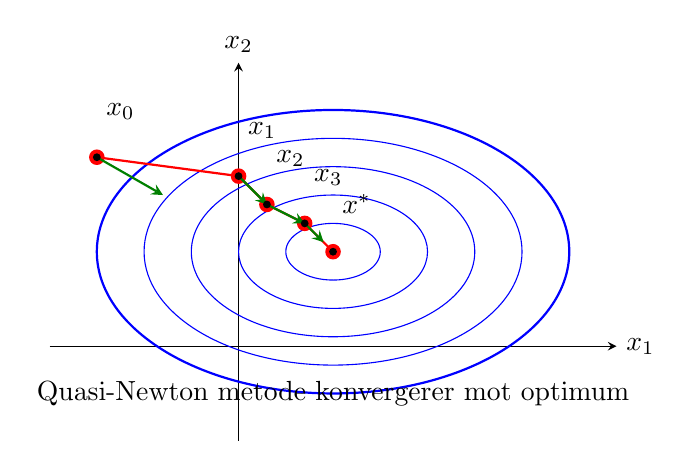
\begin{tikzpicture}[
			scale=1.2,
			>=stealth,
			point/.style={circle,fill=black,inner sep=1pt},
		]

		% Koordinatsystem
		\draw[->] (-2,0) -- (4,0) node[right]{$x_1$};
		\draw[->] (0,-1) -- (0,3) node[above]{$x_2$};

		% Elliptiske nivålinjer for en kvadratisk funksjon
		\draw[blue, thick] (1,1) ellipse (2.5 and 1.5);
		\draw[blue] (1,1) ellipse (2 and 1.2);
		\draw[blue] (1,1) ellipse (1.5 and 0.9);
		\draw[blue] (1,1) ellipse (1 and 0.6);
		\draw[blue] (1,1) ellipse (0.5 and 0.3);

		% Optimeringsbane
		\draw[mark=*, red, thick, mark size=2pt] plot coordinates {
				(-1.5, 2)
				(0, 1.8)
				(0.3, 1.5)
				(0.7, 1.3)
				(1, 1)
			};

		% Gradient piler
		\draw[->, green!50!black, thick] (-1.5, 2) -- (-0.8, 1.6);
		\draw[->, green!50!black, thick] (0, 1.8) -- (0.3, 1.5);
		\draw[->, green!50!black, thick] (0.3, 1.5) -- (0.7, 1.3);
		\draw[->, green!50!black, thick] (0.7, 1.3) -- (0.9, 1.1);

		% Legg til punkter for tydelighet
		\node[point, label={[shift={(0.3,0.3)}]$\symbf{x}_0$}] at (-1.5, 2) {};
		\node[point, label={[shift={(0.3,0.3)}]$\symbf{x}_1$}] at (0, 1.8) {};
		\node[point, label={[shift={(0.3,0.3)}]$\symbf{x}_2$}] at (0.3, 1.5) {};
		\node[point, label={[shift={(0.3,0.3)}]$\symbf{x}_3$}] at (0.7, 1.3) {};
		\node[point, label={[shift={(0.3,0.3)}]$\symbf{x}^\ast$}] at (1, 1) {};

		% Figurtittel
		\node at (1, -0.5) {Quasi-Newton metode konvergerer mot optimum};

	\end{tikzpicture}
	\caption{Illustrasjon av Quasi-Newton-iterasjoner som konvergerer mot løsningen langs en ikke-lineær vei. De elliptiske konturene representerer nivålinjer for objektfunksjonen, og punktene viser iterasjonene fra \(\symbf{x}_0\) til den optimale løsningen \(\symbf{x}^\ast\).}
	\label{fig:quasi_newton_convergence}
\end{figure}

\subsection{Limited Memory BFGS (L-BFGS)}
For høydimensjonale problemer kan det å lagre hele Hesse-approksimasjonen være vanskelig.
Limited Memory BFGS (L-BFGS) lagrer kun de siste \(m\) parene \((\symbf{s}_k, \symbf{y}_k)\) og konstruerer approksimasjonen implisitt.


\subsection{Egenskaper ved Quasi-Newton metoder}

\paragraph{Fordeler}
\begin{itemize}
	\item Raskere enn gradientbaserte metoder
	\item Lavere kostnad per iterasjon enn Newtons metode
	\item Bygger opp kurvaturinformasjon iterativt
	\item Superlineær konvergens under passende betingelser
\end{itemize}

\paragraph{Ulemper}
\begin{itemize}
	\item Langsommere konvergens enn ren Newton-metode lokalt
	\item Kan kreve flere linjesøk
	\item Sensitiv til nøyaktigheten i linjesøket, spesielt for DFP
\end{itemize}


For å sikre at Hesse-approksimasjonen forblir positiv definit, er det viktig at:

\begin{itemize}
	\item \(\symbf{y}_k^T\symbf{s}_k > 0\) (oppfylt under sterke Wolfe-betingelser)
	\item Initialmatrisen \(\symbf{B}_0\) eller \(\symbf{H}_0\) er positiv definit (ofte satt til \(\symbf{I}\))
\end{itemize}

En vanlig tilnærming for å forbedre ytelsen er å skalere den innledende approksimasjonen:

\[
	\symbf{H}_0 = \frac{\symbf{y}_k^T\symbf{s}_k}{\symbf{y}_k^T\symbf{y}_k}\symbf{I}
\]

Dette gir et bedre estimat for den faktiske skaleringen av den inverse Hesse-matrisen.

\subsection{Superlineær konvergens av Quasi-Newton metoder}

Under visse forutsetninger kan kvasi-Newton-metoder oppnå \textit{superlineær konvergens}. Dette skjer dersom søkeretningen \( \symbf{p}_k \) tilfredsstiller
\[
	\lim_{k \to \infty} \frac{\| (B_k - \nabla^2 f(\symbf{x}^\ast)) \symbf{p}_k \|}{\|\symbf{p}_k\|} = 0,
\]
hvor \( \symbf{x}_k \to \symbf{x}^\ast \) og \( \nabla^2 f(\symbf{x}^\ast) \succ 0 \). Dette innebærer at det ikke er nødvendig at \( B_k \to \nabla^2 f(\symbf{x}^\ast) \) i alle retninger – det er tilstrekkelig at tilnærmingen er god i retningen \( \symbf{p}_k \). Dette er en viktig og litt overraskende egenskap ved kvasi-Newton-metoder.

\begin{theorem}{Superlineær konvergens for kvasi-Newton}{quasi_newton_superlinear}
	La \( f : \mathbb{R}^n \to \mathbb{R} \) være to ganger kontinuerlig deriverbar. Anta at iterasjonene \( \symbf{x}_{k+1} = \symbf{x}_k + \alpha_k \symbf{p}_k \) bruker søkeretninger \( \symbf{p}_k \) som er desentrerte, og at steglengdene \( \alpha_k \) tilfredsstiller Wolfe-betingelsene med \( c_1 \le 1/2 \). Hvis \( \symbf{x}_k \to \symbf{x}^\ast \), hvor \( \nabla f(\symbf{x}^\ast) = 0 \) og \( \nabla^2 f(\symbf{x}^\ast) \) er positivt definit, og hvis
	\[
		\lim_{k \to \infty} \frac{\| \nabla f(\symbf{x}_k) + \nabla^2 f(\symbf{x}_k) \symbf{p}_k \|}{\|\symbf{p}_k\|} = 0,
	\]
	da gjelder:
	\begin{enumerate}
		\item Det finnes et \( k_0 \) slik at \( \alpha_k = 1 \) blir akseptert for alle \( k > k_0 \).
		\item Dersom \( \alpha_k = 1 \) for alle \( k > k_0 \), konvergerer \( \{\symbf{x}_k\} \) superlineært mot \( \symbf{x}^\ast \).
	\end{enumerate}
\end{theorem}

I kvasi-Newton-metoder er søkeretningen gitt ved \( \symbf{p}_k = -B_k^{-1} \nabla f_k \), og tilhørende tilstand for superlineær konvergens kan formuleres som:

\begin{theorem}{Nødvendig og tilstrekkelig betingelse for superlineær konvergens}{quasi_newton_superlinear_condition}
	Anta at \( f : \mathbb{R}^n \to \mathbb{R} \) er to ganger kontinuerlig deriverbar, og at \( \symbf{x}_k \to \symbf{x}^\ast \), der \( \nabla f(\symbf{x}^\ast) = 0 \) og \( \nabla^2 f(\symbf{x}^\ast) \) er positivt definit. Anta videre at iterasjonen er gitt ved
	\[
		\symbf{x}_{k+1} = \symbf{x}_k + \symbf{p}_k,
	\]
	hvor \( \symbf{p}_k = -B_k^{-1} \nabla f(\symbf{x}_k) \). Da konvergerer \( \{\symbf{x}_k\} \) superlineært mot \( \symbf{x}^\ast \) hvis og bare hvis
	\[
		\lim_{k \to \infty} \frac{\| (B_k - \nabla^2 f(\symbf{x}^\ast)) \symbf{p}_k \|}{\|\symbf{p}_k\|} = 0.
	\]
\end{theorem}

Dette viser at superlineær konvergens kan oppnås selv om \( B_k \not\to \nabla^2 f(\symbf{x}^\ast) \) i operatornorm - det er nok at \( B_k \) tilnærmer Hesse-matrisen godt langs retningene \( \symbf{p}_k \).

Under passende betingelser viser Quasi-Newtons metoder superlineær konvergens:

\[
	\lim_{k \to \infty} \frac{\|\symbf{x}_{k+1} - \symbf{x}^\ast\|}{\|\symbf{x}_k - \symbf{x}^\ast\|} = 0
\]
Selv om denne konvergensraten er langsommere enn Newtons kvadratiske konvergens, er kostnaden per iterasjon betydelig lavere, noe som gir en mer effektiv algoritme totalt sett, spesielt for store problemer.

\chapter{Optimal Steglengde \texorpdfstring{\(\alpha\)}{alpha}}
\label{chap:step_length_methods}
Steglengdemetoder er en viktig del av optimeringsalgoritmer, spesielt i gradientbaserte metoder som Newtons metode og Quasi-Newton-metoder.

De har som mål å bestemme den optimale steglengden \(\alpha\) for å minimere objektfunksjonen \(f\) langs en gitt retning \(p\).

Disse metodene er avgjørende for å sikre at algoritmen konvergerer mot en løsning på en effektiv måte.

\section{Linjesøk Metoder}
Linjesøk har som mål å finne en optimal steglengde \(\alpha_k\) i en gitt retning \(p_k\) for å minimere objektfunksjonen \(f\).

\begin{definition}{Linjesøk}{line_search}
	Gitt en nåværende iterasjon \(x_k\) og en søkeretning \(p_k\), finner linjesøk en steglengde \(\alpha_k > 0\) slik at
	\[
		x_{k+1} = x_k + \alpha_k p_k
	\]
	gir tilstrekkelig reduksjon i \(f\) langs retningen \(p_k\).
\end{definition}

For å oppnå dette, må vi oppfylle visse betingelser for \(\alpha_k\).
De varierer i hvor strenge krav de stiller til reduksjonen i funksjonsverdien, gradientens/Hesse-matrisens oppførsel og forholdet mellom disse.
De mest kjente er Wolfe-betingelsene, Armijo-betingelsen, Goldstein-betingelsen, kurvbetingelsen og Strong Wolfe-betingelsene.

\subsection{Wolfe-betingelsene}
Wolfe-betingelsene er en samling av betingelser som sikrer at linjesøket gir tilstrekkelig reduksjon i funksjonsverdien og at gradienten ikke endrer retning for brått.


\begin{align}
	f(x_k + \alpha_k p_k)              & \leq f(x_k) + c_1 \alpha_k \nabla f(x_k)^T p_k \tag{Armijo betingelse} \\
	\nabla f(x_k + \alpha_k p_k)^T p_k & \geq c_2 \nabla f(x_k)^T p_k \tag{Krumningsbetingelse}
\end{align}

der \(0 < c_1 < c_2 < 1\) er konstanter, typisk \(c_1 \approx 10^{-4}\) og \(c_2 \approx 0.9\).

\begin{definition}{Wolfe-betingelsene}{wolfe_conditions}
	\textbf{Armijo-betingelsen}:
	\begin{align*}
		f(\symbf{x} + \alpha \symbf{d})                    & \le f(\symbf{x}) + \beta\,\alpha\,\nabla f(\symbf{x})^T \symbf{d} \tag{Armijo} \\
		\nabla f(\symbf{x} + \alpha \symbf{d})^T \symbf{d} & \ge \rho \,\nabla f(\symbf{x})^T \symbf{d} \tag{Krumningsbetingelse}
	\end{align*}
\end{definition}

\begin{lemma}{Well-posedness av Wolfe-betingelsene}{well_posedness_wolfe_conditions}
	Anta at \(f:\R^n \to \R \) er kontinuerlig deriverbar. La \(\mathbf{p}_k\) være nedstigningsretningen ved iterasjon \(\mathbf{x}_k\), og anta at \(f\) er bundet nedenfra langs strålen:

	\[
		\{\mathbf{x}_k + \alpha \mathbf{p}_k : \alpha > 0\} \subset \mathbb{R}^n.
	\]

	\medskip

	Hvis \(0 < c_1 < c_2 < 1\), så eksisterer det intervaller av steglengder \(\alpha_k > 0\) slik at både Wolfe-betingelsene~\ref{def:wolfe_conditions} og Strong Wolfe-betingelsene~\ref{def:strong_wolfe_conditions} er oppfylt.

\end{lemma}

\subsection{Armijo-betingelsen}
\begin{definition}{Armijo-betingelsen}{armijo_condition}
	Armijo-betingelsen sikrer at steget gir en tilstrekkelig reduksjon i funksjonsverdien. Den krever at
	\[
		f(\symbf{x} + \alpha \symbf{d})
		\;\le\;
		f(\symbf{x})
		\;+\;
		\beta\,\alpha\,\nabla f(\symbf{x})^T \symbf{d},
	\]
	hvor \(\beta\) er en liten positiv konstant. Dette tilsier at \(f\) reduseres i tråd med en lineær modell.
\end{definition}

\begin{figure}[H]
	\centering
	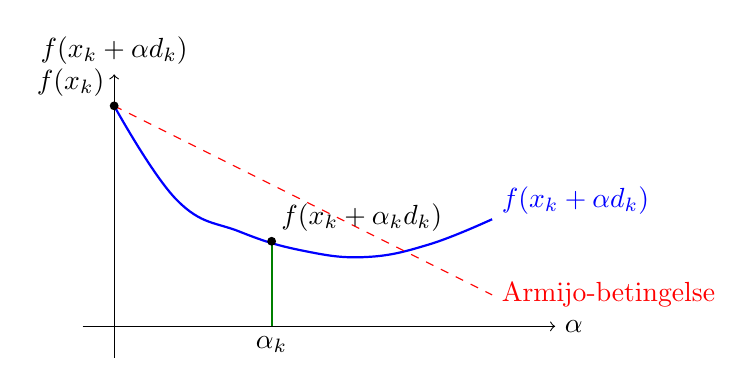
\begin{tikzpicture}[scale=0.8]
		% Axis
		\draw[->] (-0.5,0) -- (7,0) node[right]{$\alpha$};
		\draw[->] (0,-0.5) -- (0,4) node[above]{$f(\symbf{x}_k + \alpha \symbf{d}_k)$};

		% Function curve
		\draw[thick, blue] plot[smooth, tension=0.7] coordinates {(0,3.5) (1,2) (2,1.5) (3,1.2) (4,1.1) (5,1.3) (6,1.7)};

		% Armijo condition line
		\draw[red, dashed] plot coordinates {(0,3.5) (6,0.5)};

		% Initial point
		\fill (0,3.5) circle (2pt) node[above left]{$f(\symbf{x}_k)$};

		% Step point
		\draw[green!50!black, thick] (2.5,0) -- (2.5,1.35);
		\fill (2.5,1.35) circle (2pt) node[above right]{$f(\symbf{x}_k + \alpha_k \symbf{d}_k)$};

		% Step length label
		\node[below] at (2.5,0) {$\alpha_k$};

		% Legend
		\node[blue, right] at (6,2) {$f(\symbf{x}_k + \alpha \symbf{d}_k)$};
		\node[red, right] at (6,0.5) {Armijo-betingelse};
	\end{tikzpicture}
	\caption{Illustrasjon av linjesøk. Den blå kurven viser funksjonen langs søkeretningen, mens den røde stiplede linjen viser Armijo-betingelsen. Steglengden $\alpha_k$ gir tilstrekkelig reduksjon.}
\end{figure}

\subsection{Goldstein-betingelsen}
\begin{definition}{Goldstein-betingelsen}{goldstein_condition}
	Goldstein-betingelsen krever at den nye funksjonsverdien etter steget ligger innenfor et avgrenset intervall:
	\[
		f(\symbf{x}) + (1-\beta)\,\alpha\,\nabla f(\symbf{x})^T \symbf{d}
		\;\le\;
		f(\symbf{x} + \alpha \symbf{d})
		\;\le\;
		f(\symbf{x}) + \beta\,\alpha\,\nabla f(\symbf{x})^T \symbf{d}.
	\]
	Dette forhindrer at vi tar et for lite eller for stort steg.
\end{definition}

\subsection{Kurvbetingelsen}
\begin{definition}{Curvature condition}{curvature_condition}
	Kurvbetingelsen ser på gradientens endring \(\nabla f\) etter steget \(\alpha\) og krever at:
	\[
		\abs*{\nabla f(\symbf{x} + \alpha \symbf{d})^T \symbf{d}} \le -\sigma \nabla f(\symbf{x})^T \symbf{d},
	\]
	for en konstant \(\sigma \in (0,1)\). Dette sikrer at gradienten ikke endrer retning for brått, og at man unngår “overkorrigering”.
\end{definition}

\subsection{Sterk Wolfe-betingelsene}
\begin{definition}{Strong Wolfe-betingelsene}{strong_wolfe_conditions}
	Strong Wolfe-betingelsene kombinerer Armijo-betingelsen\ref{def:armijo_condition} med kurvbetingelsen\ref{def:curvature_condition} slik at:
	\begin{align*}
		f(\symbf{x} + \alpha \symbf{d})                    & \leq f(\symbf{x}) + c_1 \alpha \nabla f(\symbf{x})^T \symbf{d} \\
		\nabla f(\symbf{x} + \alpha \symbf{d})^T \symbf{d} & = c_2 \nabla f(\symbf{x})^T \symbf{d}
	\end{align*}

	der \(0 < c_1 < c_2 < 1\) er konstanter, typisk \(c_1 \approx 10^{-4}\) og \(c_2 \approx 0.9\).
	\medskip
	Disse betingelsene sikrer at steget gir tilstrekkelig reduksjon i funksjonsverdien og at gradienten ikke endrer retning for brått.
\end{definition}

\subsection{Goldstein-Wolfe-betingelsene}
\begin{definition}{Goldstein-Wolfe-betingelsene}{goldstein_wolfe_conditions}
	Goldstein-Wolfe-betingelsene krever at Armijo- og Goldstein-betingelsene begge er oppfylt:
	\begin{enumerate}
		\item Armijo-betingelsen:
		      \[
			      f(\symbf{x} + \alpha \symbf{d})
			      \;\le\;
			      f(\symbf{x})
			      \;+\;
			      \beta\,\alpha\,\nabla f(\symbf{x})^T \symbf{d}.
		      \]
		\item Goldstein-betingelsen:
		      \[
			      f(\symbf{x}) + (1-\beta)\,\alpha\,\nabla f(\symbf{x})^T \symbf{d}
			      \;\le\;
			      f(\symbf{x} + \alpha \symbf{d})
			      \;\le\;
			      f(\symbf{x}) + \beta\,\alpha\,\nabla f(\symbf{x})^T \symbf{d}.
		      \]
	\end{enumerate}
\end{definition}

\begin{figure}[H]
	\centering
	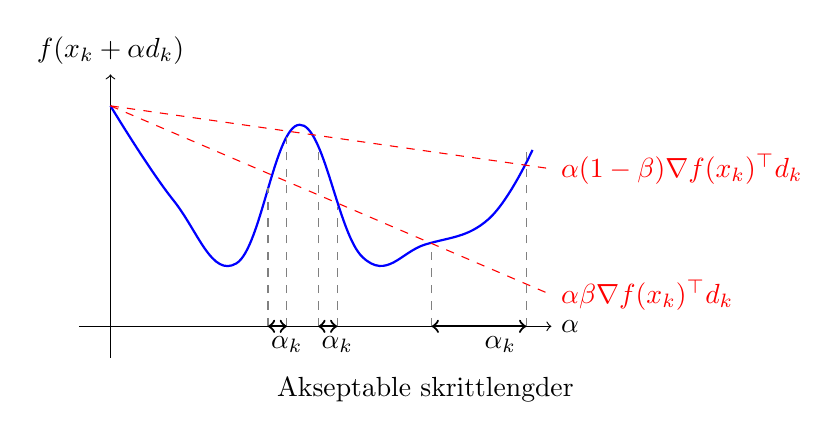
\begin{tikzpicture}[scale=0.8]
		% Akser
		\draw[->] (-0.5,0) -- (7,0) node[right]{$\alpha$};
		\draw[->] (0,-0.5) -- (0,4) node[above]{$f(\symbf{x}_k + \alpha \symbf{d}_k)$};

		% Funksjonskurve
		\draw[thick, blue] plot[smooth, tension=0.7] coordinates {(0,3.5) (1,2) (2,1) (3,3.2) (4,1.1) (5,1.3) (6,1.7) (6.7,2.8)};

		% Armijo øvre grense linje
		\draw[red, dashed] plot coordinates {(0,3.5) (7,0.5)} node[right]{$\alpha \beta \nabla f(\symbf{x}_k)^\top \symbf{d}_k$};
		% Goldstein øvre grense linje
		\draw[red, dashed] plot coordinates {(0,3.5) (7,2.5)} node[right]{$\alpha (1 - \beta) \nabla f(\symbf{x}_k)^\top \symbf{d}_k$};

		% Akseptable skrittlengder
		\draw[gray, dashed] (2.5,0) -- (2.5,2.2);
		\draw[gray, dashed] (2.8,0) -- (2.8,3.0);
		\draw[<->, thick] (2.5,0) -- (2.8,0) node[below]{$\alpha_k$};

		\draw[gray, dashed] (3.3,0) -- (3.3,2.8);
		\draw[gray, dashed] (3.6,0) -- (3.6,1.9);
		\draw[<->, thick] (3.3,0) -- (3.6,0) node[below]{$\alpha_k$};

		\draw[gray, dashed] (5.1,0) -- (5.1,1.2);
		\draw[gray, dashed] (6.6,0) -- (6.6,2.8);
		\draw[<->, thick] (5.1,0) -- (6.6,0) node[below left]{$\alpha_k$};

		% Legende
		\node at (5, -1) {Akseptable skrittlengder};



	\end{tikzpicture}
	\caption{Visualisering av Goldstein-Wolfe betingelsene.
		De akseptable skrittlengdene $\alpha$ ligger i området der funksjonen (blå kurve) er mellom Goldstein nedre grense og Armijo øvre grense (rød stiplet linje).}
	\label{fig:goldstein_wolfe_conditions}
\end{figure}

\subsection{Eksakt vs Ikke-Eksakt Linjesøk}

\begin{itemize}
	\item \textbf{Eksakt linjesøk}: Finn $\alpha_k$ som minimerer $f(x_k + \alpha p_k)$. Dette er ofte beregningsmessig dyrt.
	\item \textbf{Ikke-eksakt linjesøk}: Finn $\alpha_k$ som gir tilstrekkelig reduksjon, f.eks. ved å oppfylle Wolfe betingelsene.
\end{itemize}

Linjesøk omfatter metoder for å finne en egnet skrittlengde \(\alpha\) eller \(\alpha_k\) i en gitt retning \(\symbf{d}\) som reduserer objektfunksjonen \(f(\symbf{x})\).

\subsection{Backtracking Line Search}
Backtracking Line Search er en metode for å finne en passende skrittlengde \(\alpha\) som sikrer en ønsket reduksjon i \(f(\symbf{x})\) langs en retning \(\symbf{d}\).

\subsubsection{Algoritme}
\begin{algorithm}[H]
	\SetAlgoLined
	\KwIn{Startpunkt \( \symbf{x} \), retning \( \symbf{d} \), initial skrittlengde \( \alpha \), \textit{backtracking}-parameter \( \beta \in (0,1) \), \textit{skalering} \( \rho \in (0,1) \)}
	\KwOut{Skrittlengde \( \alpha \)}
	\While{\( f(\symbf{x} + \alpha \symbf{d}) > f(\symbf{x}) + \beta \,\alpha \,\nabla f(\symbf{x})^T \symbf{d} \)}{
		\(\alpha \leftarrow \rho \,\alpha\)
	}
	\caption{Backtracking Line Search (BLS)}
	\label{alg:backtracking_line_search}
\end{algorithm}

\subsection{Konvergens av Linjesøk}
\begin{theorem}{Konvergens av linjesøk}{line_search_convergence}
	Anta at \(f\) er kontinuerlig deriverbar og at det finnes en \(\alpha^\ast > 0\) slik at
	\[
		f(\symbf{x} + \alpha^\ast \symbf{d}) < f(\symbf{x}) + \beta\,\alpha^\ast\,\nabla f(\symbf{x})^T \symbf{d}.
	\]
	Da vil Backtracking Line Search konvergere til en skrittlengde \(\alpha_k\) som tilfredsstiller Armijo-betingelsen.
\end{theorem}

\begin{theorem}{Zoutendijk's result}{zoutendijk_result}
	La \( \symbf{x}_{k+1} = \symbf{x}_k + \alpha_k \symbf{p}_k \), hvor \( \mathbf{p}_k \) er en nedstigningsretning, med skrittlengde \( \alpha_k \) som tilfredsstiller Wolfe-betingelsene \ref{def:wolfe_conditions}.

	Anta at:
	\begin{itemize}
		\item \(f\) er bundet nedenfra i \(\R^n\)
		\item \(f\) er kontinuerlig deriverbar på det åpne settet \(\mathcal{N}\) som inneholder nivåsettet
		      \[ \mathcal{L} = \{\symbf{x}: f(\symbf{x}) \leq f(\symbf{x}_0)\} \]
		\item \(\nabla f\) er Lipschitz-kontinuerlig på \(\mathcal{N}\), dvs. det finnes en konstant \(L > 0\) slik at
		      \[ \|\nabla f(\symbf{x}) - \nabla f(\tilde{\symbf{x}})\| \leq L\|\symbf{x} - \tilde{\symbf{x}}\| \quad \text{for alle } \symbf{x}, \tilde{\symbf{x}} \in \mathcal{N} \]
	\end{itemize}

	Da har vi at:
	\[
		\sum_{k=0}^{\infty} \cos^2 \theta_k \| \nabla f(\symbf{x}_k) \|^2 < \infty,
	\]
	hvor \( \theta_k \) er vinkelen mellom \( \nabla f(\symbf{x}_k) \) og søkeretningen \( \symbf{p}_k \).

	Dette innebærer at \( \| \nabla f(\symbf{x}_k) \| \to 0 \) når \( k \to \infty \).

	\medskip

	Dette resultatet viser at hvis vi har en sekvens av iterasjoner \( \{ \symbf{x}_k \} \) som tilfredsstiller Wolfe-betingelsene, og hvis nivåsettet \( \mathcal{L} \) er begrenset og lukket (kompakt), så vil gradienten konvergere mot null.

\end{theorem}

\section{Trust Region}
\label{sec:trust_region}
Trust Region metoder er en klasse av optimeringsalgoritmer som skiller seg fra linjesøkmetoder ved at de bestemmer både retning og steglengde samtidig.
Det grunnleggende prinsippet er å definere et \emph{tillitsområde} rundt den nåværende iterasjonen \(\symbf{x}_k\), hvor vi antar at den kvadratiske modellen \(m_k(\symbf{p})\) gir en god tilnærming av objektfunksjonen \(f(\symbf{x})\).

I hver iterasjon løser metoden et begrenset optimeringsproblem av formen:
\[
	\min_{\symbf{p} \in \mathbb{R}^n} m_k(\symbf{p}) = f_k + \symbf{g}_k^T\symbf{p} + \frac{1}{2}\symbf{p}^T\symbf{B}_k\symbf{p} \quad \text{slik at} \quad \|\symbf{p}\| \leq \Delta_k
\]
hvor:
\begin{itemize}
	\item $f_k = f(\symbf{x}_k)$ er funksjonsverdien i nåværende punkt
	\item $\symbf{g}_k = \nabla f(\symbf{x}_k)$ er gradienten
	\item $\symbf{B}_k$ er en symmetrisk matrise som approksimerer Hesse-matrisen $\nabla^2 f(\symbf{x}_k)$
	\item $\Delta_k$ er radiusen til tillitsområdet
\end{itemize}

For optimeringsproblemer på formen \eqref{eq:unconstrained_optimization_problem} gir denne tilnærmingen flere fordeler:
\begin{itemize}
	\item Vi kan kontrollere kvaliteten på modellen ved å justere størrelsen på tillitsområdet
	\item Metoden kan håndtere ikke-konvekse problemer mer robust enn linjesøkmetoder
	\item Den kvadratiske modellen gir god lokal tilnærming når vi er nær et minimum
\end{itemize}


\begin{definition}{Trust Region}{trust_region}
	En \textbf{trust region} er et område rundt den nåværende iterasjonen \( \symbf{x}_k \) der vi antar at den kvadratiske modellen \( m_k(\symbf{p}) \) er en tilstrekkelig representasjon av objektfunksjonen \( f(\symbf{x}) \).
	\[
		\mathcal{D}_k = \{\symbf{x} : \|\symbf{x} - \symbf{x}_k\| \leq \Delta_k\}
	\]
	hvor \( \Delta_k \) er radiusen til trust regionen.
\end{definition}

\begin{figure}[H]
	\centering
	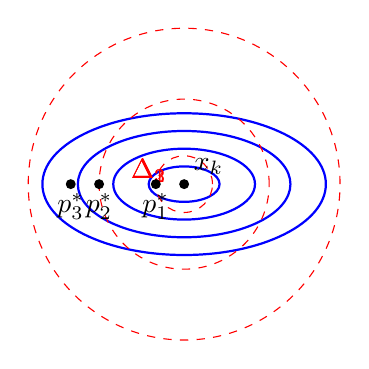
\begin{tikzpicture}[scale=0.9]
		% Konturlinjer for modellen
		\draw[blue, thick] (0,0) ellipse (2 and 1);
		\draw[blue, thick] (0,0) ellipse (1.5 and 0.75);
		\draw[blue, thick] (0,0) ellipse (1 and 0.5);
		\draw[blue, thick] (0,0) ellipse (0.5 and 0.25);

		% Forskjellige trust regions
		\draw[red, dashed] (0,0) circle (0.4) node[above left, xshift=-0.1cm, yshift=-0.1cm] {$\Delta_1$};
		\draw[red, dashed] (0,0) circle (1.2) node[above left, xshift=-0.1cm, yshift=-0.1cm] {$\Delta_2$};
		\draw[red, dashed] (0,0) circle (2.2) node[above left, xshift=-0.1cm, yshift=-0.1cm] {$\Delta_3$};

		% Nuværende punkt
		\fill (0,0) circle (2pt) node[above right] {$\symbf{x}_k$};

		% Løsningspunkter
		\fill (-0.4,0) circle (2pt) node[below] {$\symbf{p}_1^\ast$};
		\fill (-1.2,0) circle (2pt) node[below] {$\symbf{p}_2^\ast$};
		\fill (-1.6,0) circle (2pt) node[below] {$\symbf{p}_3^\ast$};

	\end{tikzpicture}
	\caption{Løsning av trust region-underproblemet for forskjellige radier $\Delta_1$, $\Delta_2$, $\Delta_3$. For liten radius ($\Delta_1$) ligger løsningen på grensen, for medium radius ($\Delta_2$) også på grensen, mens for stor radius ($\Delta_3$) er løsningen den ubegrensede minimanten.}
	\label{fig:trust_region_solutions}
\end{figure}

\subsection{Trust Region Algoritme}
Det viktigste i en trust region-algoritme er hvordan man velger trust region-radius $\Delta_k$ ved hver iterasjon. Dette valget baseres på forholdet $\rho_k$:
\[
	\rho_k = \frac{f(\symbf{x}_k) - f(\symbf{x}_k + \symbf{p}_k)}{m_k(\symbf{0}) - m_k(\symbf{p}_k)}
\]

\begin{algorithm}[H]
	\SetAlgoLined
	\KwIn{Startpunkt $\symbf{x}_0$, initial trust region radius $\Delta_0 > 0$, parametere $\hat{\Delta} > 0, \eta \in (0, \frac{1}{4})$ og $\gamma \in (0, \frac{1}{4})$}
	\KwOut{Løsning $\symbf{x}^\ast$}
	\For{$k = 0, 1, 2, \ldots$}{
		Finn steget $\symbf{p}_k$ med Cauchy- eller Dogleg-metoden.\\
		Beregn forholdet $\rho_k$.\\
		\uIf{$\rho_k < \frac{1}{4}$}{
			$\Delta_{k+1} \leftarrow \frac{1}{4}\Delta_k$
		}
		\Else{
			\uIf{$\rho_k > \frac{3}{4}$ \textbf{og} $\|\symbf{p}_k\| = \Delta_k$}{
				$\Delta_{k+1} \leftarrow \min(2\Delta_k, \hat{\Delta})$
			}
			\Else{
				$\Delta_{k+1} \leftarrow \Delta_k$
			}
		}
		\If{$\rho_k > \eta$}{
			$\symbf{x}_{k+1} \leftarrow \symbf{x}_k + \symbf{p}_k$
		}
		\Else{
			$\symbf{x}_{k+1} \leftarrow \symbf{x}_k$
		}
	}
	\caption{Trust Region Algoritme}
	\label{alg:trust_region}
\end{algorithm}

\begin{algorithm}[H]
	\SetAlgoLined
	\KwIn{Startpunkt \( x_0 \in \mathbb{R}^n \), initial radius \( \Delta_0 > 0 \), parametere \( 0 < \eta < 1 \), \( 0 < \gamma_1 < 1 < \gamma_2 \)}
	\KwOut{Løsning \( x^\ast \)}
	\For{\( k = 0, 1, 2, \dots \)}{
		Løs delproblemet for å finne et steg \( p_k \)\;
		Beregn forholdet:
		\[
			\rho_k = \frac{f(x_k) - f(x_k + p_k)}{m_k(0) - m_k(p_k)}
		\]\;
		Oppdater punktet:
		\[
			x_{k+1} = \begin{cases}
				x_k + p_k, & \rho_k \ge \eta, \\[6pt]
				x_k,       & \rho_k < \eta.
			\end{cases}
		\]\;
		Oppdater tillitsområdet:
		\[
			\Delta_{k+1} = \begin{cases}
				\gamma_2 \Delta_k, & \rho_k > \eta,       \\[6pt]
				\Delta_k,          & \rho_k \approx \eta, \\[6pt]
				\gamma_1 \Delta_k, & \rho_k < \eta.
			\end{cases}
		\]
	}
	\caption{Intuitivt øker vi tillitsområdet når modellen er god og krymper det når modellen er dårlig.}
	\label{alg:trust_region_2}
\end{algorithm}

\subsection{Tillitsområde-steg}
Stegene karakteriseres gjennom en første-ordens nødvendig optimalitetsbetingelse:
\begin{theorem}{Karakterisering av tillitsområde-steg}{trust_region_step}
	Punktet $\symbf{p}^\ast$ er løsning av trust-region delproblemet hvis og bare hvis
	\[
		(\symbf{B}_k + \lambda^\ast \symbf{I})\symbf{p}^\ast = -\nabla f(\symbf{x}_k), \quad \lambda^\ast (\Delta_k - \|\symbf{p}^\ast\|) = 0, \quad \symbf{B}_k + \lambda^\ast \symbf{I} \succeq 0, \quad \lambda^\ast \ge 0.
	\]
	Dette innebærer at enten ligger løsningen på grensen av området, eller den ligger innenfor med $\lambda^\ast = 0$.
\end{theorem}

\begin{proof}{}{}
	Hovedidéen i beviset av Teorem \ref{thm:trust_region_step} er å bruke Lagrange-multiplikatorer for å håndtere trust-region-betingelsen som en begrensning:

	\[
		\min_p m_k(p), \quad \text{s.t.} \quad \|p\|^2 - \Delta_k^2 \leq 0.
	\]

	Lagrangianen blir
	\[
		\mathcal{L}(p,\lambda) = m_k(p) + \lambda(\|p\|^2 - \Delta_k^2),
	\]
	og første-ordens betingelser leder til ligningssystemet i teoremet.
\end{proof}

\begin{theorem}{Karakterisering av Trust Region-løsningen}{trust_region_solution}
	En vektor $\symbf{p}^\ast$ er en global løsning av trust region-problemet
	\[
		\min_{\symbf{p} \in \mathbb{R}^n} m(\symbf{p}) = f + \symbf{g}^T\symbf{p} + \frac{1}{2}\symbf{p}^T\symbf{B}\symbf{p}, \quad \text{slik at} \quad \|\symbf{p}\| \leq \Delta,
	\]
	hvis og bare hvis $\symbf{p}^\ast$ er gyldig og det finnes en skalar $\lambda \geq 0$ slik at følgende betingelser er oppfylt:
	\begin{align}
		(\symbf{B} + \lambda\symbf{I})\symbf{p}^\ast & = -\symbf{g},                   \\
		\lambda(\Delta - \|\symbf{p}^\ast\|)         & = 0,                            \\
		(\symbf{B} + \lambda\symbf{I})               & \text{ er positiv semidefinit.}
	\end{align}
	hvor $\lambda \geq 0$ er en Lagrange-multiplikator.
\end{theorem}

Dette teoremet gir flere interessante tilfeller:
\begin{itemize}
	\item Når løsningen er strengt innenfor trust region ($\|\symbf{p}^\ast\| < \Delta$), har vi $\lambda = 0$ fra komplementaritetsbetingelsen, så $\symbf{B}\symbf{p}^\ast = -\symbf{g}$.
	\item Når løsningen ligger på grensen ($\|\symbf{p}^\ast\| = \Delta$), kan $\lambda > 0$, hvilket betyr at $\symbf{p}^\ast$ er kollineær med den negative gradienten av modellen.
\end{itemize}

Trust region-metoden justerer radiusen $\Delta_k$ basert på hvor godt modellen forutsier den faktiske funksjonsverdien. Dette gjøres ved å beregne forholdet:
\[
	\rho_k = \frac{f(\symbf{x}_k) - f(\symbf{x}_k + \symbf{p}_k)}{m_k(\symbf{0}) - m_k(\symbf{p}_k)}
\]

Hvis $\rho_k$ er nær 1, betyr det at modellen gir en god prediksjon, og vi kan utvide trust region-radiusen. Hvis $\rho_k$ er nær 0 eller negativ, reduserer vi radiusen siden modellen ikke er pålitelig over så store avstander.
For å karakterisere de eksakte løsningene av trust region-underproblemet, kan vi benytte følgende teorem som viser at løsningen $\symbf{p}^\ast$ tilfredsstiller:

\[
	(\symbf{B} + \lambda \symbf{I})\symbf{p}^\ast = -\symbf{g}
\]

For å bevise teoremet, har vi bruk for følgende lemma:

\begin{lemma}{Kvadratisk minimering}{quadratic_minimization}
	La \(m\) være den kvadratiske funksjonen definert ved
	\[
		m(\symbf{p}) = \symbf{g}^\top \symbf{p} + \frac{1}{2} \symbf{p}^\top \symbf{B}\symbf{p},
	\]
	hvor \(\symbf{B}\) er en symmetrisk matrise. Da gjelder følgende:
	\begin{enumerate}
		\item Hvis \(\symbf{B}\) er positiv semidefinit, er enhver \(\symbf{p}\) som tilfredsstiller \(\symbf{B}\symbf{p} = -\symbf{g}\) en global minimerer av \(m\).
		\item \(m\) oppnår et minimum hvis og bare hvis \(\symbf{B}\) er positiv semidefinit og \(\symbf{g}\) er i bildet til \(\symbf{B}\).
		\item \(m\) har en unik minimerer hvis og bare hvis \(\symbf{B}\) er positiv definit.
	\end{enumerate}
\end{lemma}

\begin{proof}{Bevis av Lemma \ref{lem:quadratic_minimization}}
	Vi beviser hver av de tre påstandene separat:

	\begin{enumerate}
		\item \textbf{Hvis \(\symbf{B}\) er positiv semidefinit, er enhver \(\symbf{p}\) som tilfredsstiller \(\symbf{B}\symbf{p} = -\symbf{g}\) en global minimerer av \(m\):}

		      Anta at \(\symbf{p}\) tilfredsstiller \(\symbf{B}\symbf{p} = -\symbf{g}\). For enhver \(\symbf{w} \in \mathbb{R}^n\) har vi:
		      \[
			      m(\symbf{p} + \symbf{w}) = m(\symbf{p}) + \symbf{w}^\top \symbf{B} \symbf{w}.
		      \]
		      Siden \(\symbf{B}\) er positiv semidefinit, følger det at \(\symbf{w}^\top \symbf{B} \symbf{w} \geq 0\). Dermed er \(m(\symbf{p} + \symbf{w}) \geq m(\symbf{p})\), og \(\symbf{p}\) er en global minimerer.

		\item \textbf{\(m\) oppnår et minimum hvis og bare hvis \(\symbf{B}\) er positiv semidefinit og \(\symbf{g}\) er i bildet til \(\symbf{B}\):}

		      \begin{itemize}
			      \item \textit{Hvis-delen:} Hvis \(\symbf{B}\) er positiv semidefinit og \(\symbf{g}\) er i bildet til \(\symbf{B}\), finnes det en \(\symbf{p}\) slik at \(\symbf{B}\symbf{p} = -\symbf{g}\). Fra punkt (1) følger det at \(m\) oppnår et minimum.
			      \item \textit{Bare hvis-delen:} Anta at \(m\) oppnår et minimum i \(\symbf{p}\). Da må \(\nabla m(\symbf{p}) = \symbf{B}\symbf{p} + \symbf{g} = 0\), som impliserer at \(\symbf{g}\) er i bildet til \(\symbf{B}\). Videre må \(\nabla^2 m(\symbf{p}) = \symbf{B}\) være positiv semidefinit for at \(\symbf{p}\) skal være et minimum.
		      \end{itemize}

		\item \textbf{\(m\) har en unik minimerer hvis og bare hvis \(\symbf{B}\) er positiv definit:}

		      \begin{itemize}
			      \item \textit{Hvis-delen:} Hvis \(\symbf{B}\) er positiv definit, er \(\symbf{B}\symbf{p} = -\symbf{g}\) et lineært system med en unik løsning. Dermed har \(m\) en unik minimerer.
			      \item \textit{Bare hvis-delen:} Anta at \(\symbf{B}\) ikke er positiv definit. Da finnes det en \(\symbf{w} \neq 0\) slik at \(\symbf{w}^\top \symbf{B} \symbf{w} = 0\). Dette impliserer at \(m(\symbf{p} + \symbf{w}) = m(\symbf{p})\), så minimereren er ikke unik, hvilket gir en motsigelse.
		      \end{itemize}
	\end{enumerate}
\end{proof}

\begin{proof}{Bevis av teorem \ref{thm:trust_region_solution}}{}
	Anta først at betingelsene er oppfylt med en \(\lambda \geq 0\). Fra Lemma \ref{lem:quadratic_minimization} følger det at \(\symbf{p}^\ast\) er et globalt minimum av \(m(\symbf{p}) + \frac{\lambda}{2} \|\symbf{p}\|^2\), og dermed også et globalt minimum av trust region-problemet.

	For motsatt retning, anta at \(\symbf{p}^\ast\) er en global løsning. Hvis \(\|\symbf{p}^\ast\| < \Delta\), er \(\symbf{p}^\ast\) en (ubundet) minimerer av \(m\), og \(\lambda = 0\) tilfredsstiller betingelsene.
	Hvis \(\|\symbf{p}^\ast\| = \Delta\), følger det fra KKT-betingelsene at det finnes en \(\lambda \geq 0\) slik at \((\symbf{B} + \lambda \symbf{I})\symbf{p}^\ast = -\symbf{g}\) og \((\symbf{B} + \lambda \symbf{I})\) er positiv semidefinit.
\end{proof}


\subsection{Cauchy-punkt}
Cauchy-punktet er det punktet langs retningen av den bratteste nedstigningen (steepest descent), som løser delproblemet enklest:

\[
	\symbf{p}_C = -\tau_k \frac{\Delta_k \nabla f(\symbf{x}_k)}{\norm*{\nabla f(\symbf{x}_k)}^2},
	\quad
	\tau_k = \frac{\norm*{\nabla f(\symbf{x}_k)}^2}{\nabla f(\symbf{x}_k)^\top \symbf{B}_k \nabla f(\symbf{x}_k)}.
\]


\subsection{Dogleg-metoden}
Dogleg--metoden kombinerer retningene fra Newton-steget og Cauchy-punktet i en brutt linje (\enquote{dogleg}).
\begin{itemize}
	\item Først langs Newton-retningen til Newton-punktet hvis det er innenfor trust-region.
	\item Ellers finner man skjæringspunktet med kanten av tillitsområdet.
\end{itemize}

\begin{figure}[H]
	\centering
	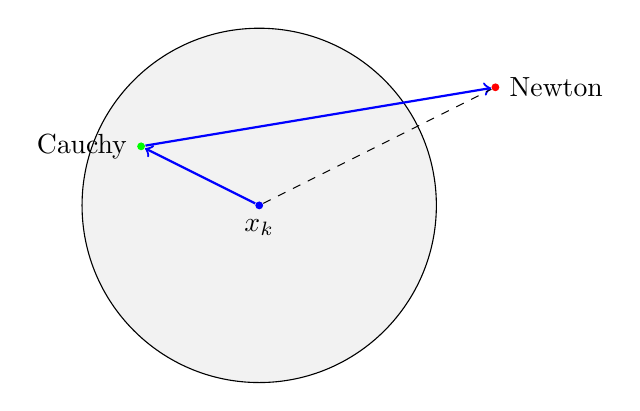
\begin{tikzpicture}[scale=1.5]
		\draw[fill=gray!10] (0,0) circle(1.5);
		\node[circle,fill=blue,inner sep=1pt,label=below:{$x_k$}] (xk) at (0,0) {};
		\node[circle,fill=red,inner sep=1pt,label=right:{Newton}] (N) at (2,1) {};
		\node[circle,fill=green,inner sep=1pt,label=left:{Cauchy}] (C) at (-1,0.5) {};
		\draw[thick,->,blue] (xk)--(C);
		\draw[thick,->,blue] (C)--(N);
		\draw[dashed] (xk)--(N);
	\end{tikzpicture}
	\caption{Dogleg-metoden kombinerer Cauchy-punktet og Newton-punktet.}
\end{figure}



\subsection{Trust Region vs Linjesøk}

\begin{itemize}
	\item \textbf{Trust region}: Først bestemmes hvor langt vi kan gå (radius \( \Omega_k \)), deretter bestemmes retningen og steglengden samtidig.
	\item \textbf{Linjesøk}: Først bestemmes retningen \( p_k \), deretter bestemmes hvor langt vi skal gå i den retningen (steplengde \( \alpha_k \)).
\end{itemize}

\chapter{Gradientfrie metoder}
\label{sec:gradientfrie_metoder}

Gradientfrie metoder er optimeringsalgoritmer som ikke benytter gradienter eller Hesse-matriser i søket etter et minimum.
De egner seg spesielt godt i situasjoner der objektfunksjonen \( f : \mathbb{R}^n \to \mathbb{R} \) er:
\begin{itemize}
	\item ikke-differensierbar eller stykkevis glatt,
	\item støyete, simulert eller svartboksbasert,
	\item kostbar eller upraktisk å derivere.
\end{itemize}

I stedet for å bruke analytisk eller numerisk informasjon om deriverte, evaluerer slike metoder funksjonsverdier i ulike retninger eller punktkombinasjoner, og gjør fremskritt basert på hvilke punkter som gir forbedring.

Gradientfrie metoder kan være svært effektive når informasjonen om objektfunksjonen er begrenset. De gir imidlertid sjelden noen garanti for å finne et globalt minimum, eller for konvergens i klassisk forstand.

\subsection{Heuristiske metoder}

En heuristisk metode er en algoritme som forsøker å finne en god (men ikke nødvendigvis optimal) løsning ved å bruke forenklede regler, prøve-og-feile-strategier eller strategier inspirert av natur og erfaring.

De er spesielt utviklet for problemer der klassiske metoder feiler - for eksempel når funksjonen har mange lokale minima, er ikke-glatt, støyete eller kun tilgjengelig gjennom simulering.

\paragraph{Egenskaper ved heuristiske metoder}

\begin{itemize}
	\item Utfører ofte globalt søk (f.eks. gjennom tilfeldige steg eller populasjoner).
	\item Krever ikke deriverte eller Hessian.
	\item Har lav til moderat regnekostnad.
	\item Mangler garanti for optimalitet, men gir ofte svært gode løsninger i praksis.
\end{itemize}

\subsection{Nelder--Mead-algoritmen}
\label{sec:nelder_mead}

Nelder--Mead er en populær algoritme  for å minimere funksjoner uten å bruke gradienter eller Hesse-matriser.
Den er særlig nyttig når funksjonen er \emph{ikke-glatt}, \emph{støyete} eller \emph{utilgjengelig i lukket form}.

Algoritmen bruker et \textbf{simplex}~\ref{def:simplex} (et geometrisk objekt med \( n+1 \) hjørner i \( n \)-dimensjonalt rom) i \( \mathbb{R}^n \) for å iterativt søke mot et lokalt minimum.

\begin{minipage}[t]{0.56\textwidth}
	Metoden manipulerer simplexen ved hjelp av \textbf{4 operasjoner}:
	\noindent
	\begin{itemize}
		\item \emph{Refleksjon}: Speiler det dårligste punktet gjennom tyngdepunktet
		\item \emph{Ekspansjon}: Strekker simplekset i lovende retninger
		\item \emph{Kontraksjon}: Krymper simplekset når refleksjon ikke gir forbedring
		\item \emph{Krymping}: Reduserer hele simplekset mot beste punkt
	\end{itemize}
	Gjennom disse operasjonene tilpasser simplekset seg automatisk til funksjonens form og \enquote{Kryper} mot det lokale minimum uten behov for deriverte.
\end{minipage}
\hfill
\begin{minipage}[t]{0.40\textwidth}
	\begin{figure}[H]
		\centering
		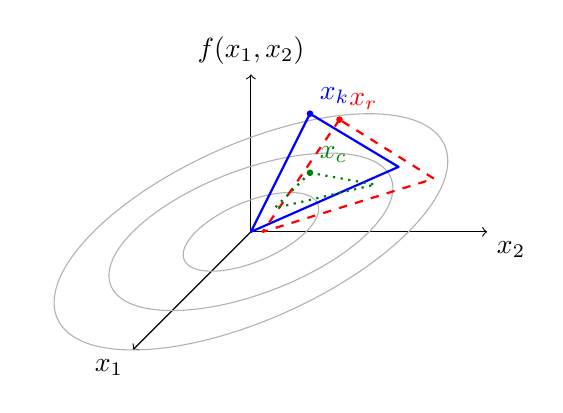
\begin{tikzpicture}[
				scale=1.0,
				x={(-0.5cm,-0.5cm)},
				y={(1cm,0cm)},
				z={(0cm,1cm)},
				line join=round
			]

			% Axes
			\draw[->] (0,0,0) -- (3,0,0) node[anchor=north east] {$x_1$};
			\draw[->] (0,0,0) -- (0,3,0) node[anchor=north west] {$x_2$};
			\draw[->] (0,0,0) -- (0,0,2) node[anchor=south] {$f(x_1,x_2)$};

			% Contours on base 
			\draw[black!30] (0,0,0) ellipse (3 and 2);
			\draw[black!30] (0,0,0) ellipse (2 and 1.5);
			\draw[black!30] (0,0,0) ellipse (1 and 0.7);

			% Initial simplex (blue solid) - scaled up by 1.5
			\draw[blue, thick]
			(1.5,1.5,2.25) -- (3,1.5,1.5) -- (2.25,3,1.95) -- cycle;

			% Reflected simplex (red dashed) - scaled up by 1.5
			\draw[red, thick, dashed]
			(0.75,1.5,1.8) -- (2.7,1.5,1.35) -- (1.65,3.15,1.5) -- cycle;

			% Contracted simplex (green dotted) - scaled up by 1.5
			\draw[green!50!black, thick, dotted]
			(1.8,1.65,1.65) -- (2.4,1.5,1.5) -- (1.95,2.55,1.575) -- cycle;

			% Key points only - scaled up by 1.5
			\fill[blue] (1.5,1.5,2.25) circle (1.2pt) node[above right] {$x_k$};
			\fill[red] (0.75,1.5,1.8) circle (1.2pt) node[above right] {$x_r$};
			\fill[green!50!black] (1.8,1.65,1.65) circle (1.2pt) node[above right] {$x_c$};

		\end{tikzpicture}
		\caption{Nelder-Mead algoritmen: Initialt (blå), reflektert (rød) og kontrahert (grønn) simplex med objektfunksjonens nivålinjer.}
		\label{fig:nelder_mead_3d}
	\end{figure}
\end{minipage}


\begin{algorithm}[H]
	\caption{Nelder--Mead-algoritme}
	\label{alg:nelder-mead}
	Initialiser simplex med \( n+1 \) punkter\;
	\Repeat{konvergenskriteriene er oppfylt}{
		Sorter simplex-punktene etter deres funksjonsverdi \( f(x_i) \)\;
		Beregn tyngdepunktet av de \( n \) beste punktene\;
		Reflekter det dårligste punktet gjennom tyngdepunktet for å få et nytt punkt \( x_r \)\;
		\uIf{\( f(x_1) \leq f(x_r) < f(x_n) \)}{
			Aksepter refleksjonen \( x_{n+1} \leftarrow x_r \)\;
		}
		\uElseIf{\( f(x_r) < f(x_1) \)}{
			Prøv ekspansjon til punkt \( x_e \)\;
			\If{\( f(x_e) < f(x_r) \)}{
				\( x_{n+1} \leftarrow x_e \)\;
			}
			\Else{
				\( x_{n+1} \leftarrow x_r \)\;
			}
		}
		\uElseIf{\( f(x_r) \geq f(x_n) \)}{
			Utfør en kontraksjon for å få punkt \( x_c \)\;
			\If{\( f(x_c) < f(x_{n+1}) \)}{
				\( x_{n+1} \leftarrow x_c \)\;
			}
			\Else{
				Krymp hele simplexet mot det beste punktet \( x_1 \)\;
			}
		}
	}
\end{algorithm}


\subsection{Andre gradientfrie metoder}

I tillegg til Nelder-Mead finnes det flere andre gradientfrie metoder:

\begin{itemize}
	\item \textbf{Genetiske algoritmer}: Inspirert av naturlig seleksjon, bruker populasjoner av løsninger som "evolusjonerer" over generasjoner.
	\item \textbf{Partikkelsverm-optimalisering (PSO)}: Inspirert av sosial atferd i fugleflokker eller fiskestimer, hvor partikler beveger seg i søkerommet.
	\item \textbf{Simulert annealing}: Inspirert av metallets varmebehandling, tillater algoritmen å akseptere dårligere løsninger med en viss sannsynlighet for å unngå å bli fanget i lokale minima.
\end{itemize}
